\PassOptionsToPackage{table}{xcolor}
\documentclass[fleqn,10pt]{wlscirep}
\usepackage[utf8]{inputenc}
\usepackage[T1]{fontenc}
\usepackage{bm}
\usepackage{colortbl}
\usepackage{booktabs}
\usepackage{tabularx}
\usepackage{array}
\usepackage{makecell}
\usepackage{graphicx}
\usepackage{subcaption}
\usepackage[normalem]{ulem}

\newcommand{\mainfigmaxheight}{0.9\textheight}
\newcommand{\old}[1]{\sout{#1}}
\newcommand{\new}[1]{{\color{red}#1}}
\newcolumntype{Y}{>{\raggedright\arraybackslash}X}
\newcommand{\erank}{\operatorname{erank}}

\definecolor{NCHeader}{HTML}{DEDCCB}
\definecolor{NCRowA}{HTML}{F1EFE7}
\definecolor{NCRowB}{HTML}{FBFBF8}
\definecolor{NatHead}{RGB}{245,246,247}
\definecolor{NatLoRA}{RGB}{232,242,248}
\definecolor{NatTT}{RGB}{244,239,249}
\definecolor{NatLRTT}{RGB}{238,248,241}
\definecolor{NatLRTTvTwo}{RGB}{255,247,230}
\definecolor{NatRule}{RGB}{115,115,115}
\definecolor{HeadGray}{RGB}{245,245,245}
\definecolor{LoRACol}{RGB}{232,246,255}
\definecolor{TTCol}{RGB}{245,236,255}
\definecolor{LRTTCol}{RGB}{235,255,238}

\title{Low-Rank Tiki-Taka: Memory-efficient transformer on-chip training for analog in-memory computing}

\author[1,3]{Young Woon Cho}
\author[1,3]{Jaeweon Park}
\author[1,2,3]{Jongun Won}
\author[1,*]{Sangbum Kim}

\affil[1]{Department of Materials Science and Engineering,
Inter-University Semiconductor Research Center, and Research Institute
of Advanced Materials, Seoul National University, Seoul 08826,
Republic of Korea}

\affil[2]{University of Notre Dame, Notre Dame, IN 46556, USA}

\affil[3]{These authors contributed equally.}

\affil[*]{e-mail: sangbum.kim@snu.ac.kr}

\begin{abstract}
As transformer models continue to scale, task adaptation becomes increasingly expensive, particularly for on-chip use. Parameter-efficient methods such as LoRA reduce the trainable state while preserving downstream-task performance, but the hardware burden remains because large dense projections are still stored and repeatedly executed, making analog in-memory computing (AIMC) attractive for parallel matrix--vector multiplication. Tiki-Taka mitigates analog update non-idealities through core--auxiliary learning, but its full-dimensional auxiliary state remains costly at transformer scale. Here we introduce Low-Rank Tiki-Taka (LR-TT), which replaces the full-size auxiliary state of Tiki-Taka with low-rank \(A/B\) auxiliary tiles. Projected updates accumulate on these tiles and are periodically consolidated via rank-wise transfer into a core tile, replacing Tiki-Taka's selected row- or column-wise transfer. Measured 6T1C synaptic arrays---with near-linear symmetric updates, \(\sim 10^3\) programmable states, and \(>10^9\)-pulse endurance---provide a suitable substrate for the auxiliary path. Hardware-in-the-loop regression and MNIST experiments validate the accumulate-and-transfer dynamics. In BERT-base fine-tuning evaluations on SQuAD v1.1, LR-TT retains performance close to full-dimensional Tiki-Taka while substantially reducing auxiliary-path energy and mapped hardware footprint. This establishes a practical route toward AIMC-based on-chip transformer adaptation beyond inference-only or digital-adapter demonstrations.

\end{abstract}
\keywords{low-rank adaptation; Tiki-Taka; analog in-memory computing; on-chip training; transformers}

\begin{document}
\emergencystretch=3em
\flushbottom
\maketitle
\thispagestyle{empty}

\noindent\textbf{Keywords:} low-rank adaptation; Tiki-Taka; analog in-memory computing; on-chip training; transformers

\section{Introduction}
\label{sec:introduction}

\begin{figure*}[t]
  \centering
  \includegraphics[width=0.9\textwidth]{Figure1.png}
  \caption{\textbf{Low-rank core/auxiliary update scheme of LR-TT.}
  (a) During each training step, the input activation is propagated primarily through the core \(C\) tile, which defines the forward path, while gradient is accumulated on the low-rank auxiliary \(A\) and \(B\) tiles by stochastic pulse updates. The $B$ tile is read to generate the projected signal used to update $A$, whereas the $A$ tile is read to generate the projected signal used to update $B$, thereby confining the auxiliary update to a rank-$r$ subspace.
 (b) At every transfer interval \(\tau\), the accumulated \(A/B\) states are read out one rank at a time using one-hot selection vectors, and the resulting rank-1 contributions are transferred to the core \(C\) tile through stochastic pulse updates.}
  \label{fig:lrtt_concept}
\end{figure*}

\begin{figure*}[!t]
  \centering
  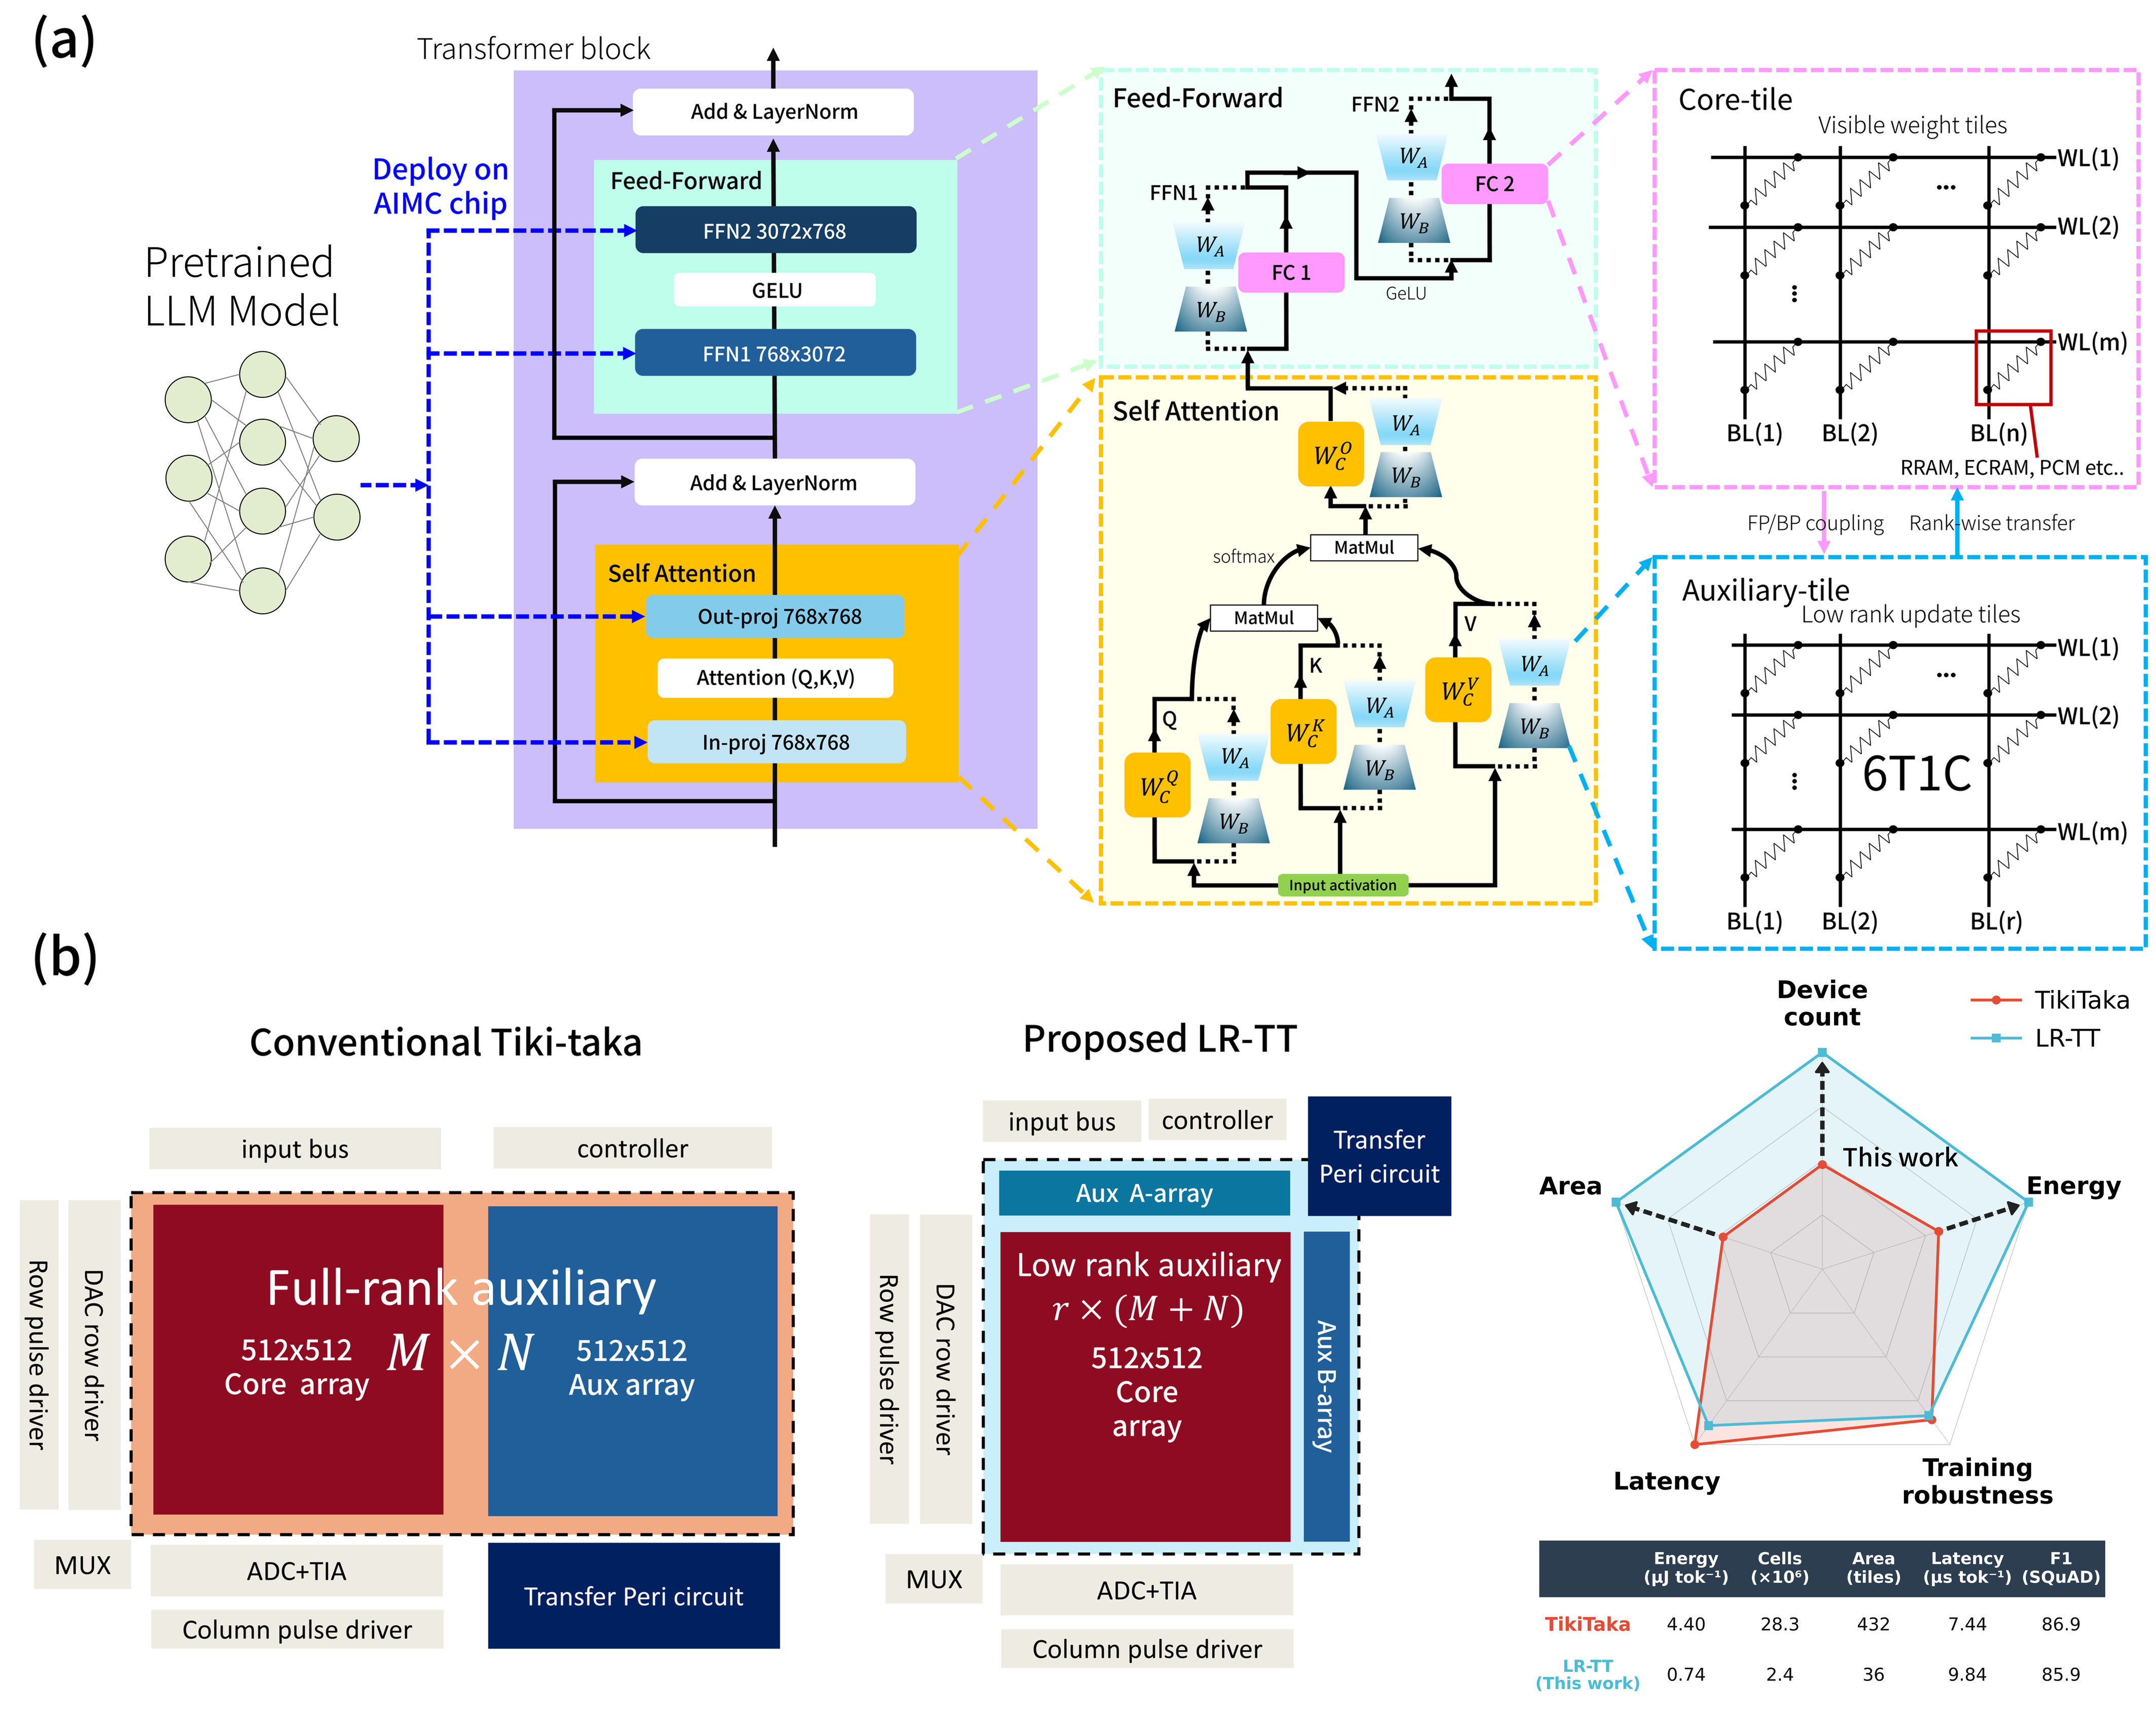
\includegraphics[width=0.9\textwidth]{Figure2.png}
  \caption{\textbf{Implementation of LR-TT for a transformer block on analog compute-in-memory hardware.}
  (a) A pretrained BERT-base model is fine-tuned on AIMC hardware, with the same mapped block structure repeated across its 12 encoder layers. In each block, the attention input projection, attention output projection, FFN1, and FFN2 linear layers are mapped to AIMC tiles, whereas attention computation, LayerNorm, and other non-matrix operations remain in digital compute. For each mapped linear operator, the core \(C\) tile stores the weight used for forward matrix--vector multiplication, while the auxiliary low-rank \(A/B\) tiles accumulate the update state and periodically transfer it to the core tile through rank-wise on-chip transfer. (b) Compared with conventional Tiki-Taka, LR-TT replaces the full-dimensional auxiliary update state with low-rank \(A/B\) tiles, thereby substantially reducing update-path energy, mapped cell count, and tile footprint. Despite this strong hardware compression, LR-TT preserves effective fine-tuning, incurring only a modest increase in token latency and a limited loss in downstream accuracy.}
  \label{fig:lrtt_transformer_mapping}
\end{figure*}

\noindent
Conventional AI accelerators face the von Neumann bottleneck: large weight matrices must be repeatedly moved between memory and processing units, incurring substantial latency and energy costs \cite{horowitz2014computing,sze2017efficient}.
This cost grows with model scale and is particularly pronounced for transformer architectures, whose large dense projections impose substantial data-movement demands during inference and adaptation \cite{vaswani2017attention,ding2023delta}.
Analog in-memory computing (AIMC) addresses this bottleneck by performing matrix--vector multiplications (MVMs) directly in memory arrays, allowing weights to remain stationary during computation \cite{ielmini2018imc,wan2022neurram,rasch2024fastrobust}.

\noindent
Most AIMC demonstrations to date have focused on inference \cite{aguirre2024memristor_ann_review,wan2022neurram,chen2025albertanalog}.
Recent work on transformer workloads has explored post-training optimization \cite{lammie2024pt_roberta}, analog inference demonstrations \cite{chen2025albertanalog}, hardware-aware adaptation with external digital low-rank adapters \cite{li2026ahwa_lora}, and architecture-level acceleration \cite{leroux2025aimc_attention,buchel2025moe_3d_aimc}.
These studies address inference or external digital adaptation rather than pulsed weight updates performed in analog arrays.
Pulsed in-memory training has instead been demonstrated on smaller networks, including convolutional models, edge-scale transfer learning, and a compact Vision Transformer evaluated in simulation \cite{ambrogio2018analogtraining,li2018insitu,wang2019insitu,ando2025transfer,rasch2024fastrobust}.
Scaling pulsed in-memory training to transformer language models such as BERT-base (\(\sim\)110\,M parameters) therefore remains an open challenge \cite{devlin2019bert}.
Such a capability would enable local adaptation of deployed models under tight energy, latency, and memory constraints, an important use case for on-chip training at the edge \cite{gokmen2016rpu,zhou2019edgeintelligence}.

\noindent
Analog in-memory training introduces device- and algorithm-level requirements beyond those of inference.
At the device level, training adds repeated local weight updates to the forward and backward MVMs \cite{gokmen2016rpu,ambrogio2018analogtraining,rasch2024fastrobust}, placing stringent demands on incremental update linearity and symmetry, state resolution, retention across update windows, and cycling endurance \cite{gokmen2021ttv2,rasch2024fastrobust,won2023advs_6t1c}.
At the algorithmic level, residual device non-idealities can bias the effective gradient, impose finite update granularity, and perturb the intended optimization trajectory \cite{ambrogio2018analogtraining,wu2025responsefunctions,rasch2024fastrobust}.
Algorithms designed for full-precision digital weight updates therefore do not account for the pulsed, non-ideal update dynamics of AIMC hardware.

\noindent
These requirements have been addressed through complementary device and algorithm advances.
On the device side, low-leakage IGZO-TFT/capacitor synaptic arrays such as 6T1C have demonstrated linear and symmetric incremental updates, retention over the relevant transfer window, and stable operation after \(10^{9}\) update pulses \cite{won2023advs_6t1c}.
Recent circuit- and array-level studies further report hundreds of programmable states \cite{kang2025jssc_6t1c}, disturbance-aware parallel update operation \cite{kang2025advs_disturbance}, and improved bias-stress reliability \cite{han2025acsami_gi}.
On the algorithm side, Tiki-Taka mitigates the effects of device non-idealities by separating gradient accumulation from weight storage across core and auxiliary arrays: an auxiliary array accumulates parallel outer-product updates, and its state is periodically transferred to a core array that stores the model weights, thereby relaxing the update-symmetry requirement of direct analog SGD \cite{gokmen2020tikitaka,onen2022asymmetric}.
TTv2 and later variants introduce digital filtering, thresholded transfer, dynamic reference estimation, and zero-point compensation \cite{gokmen2021ttv2,rasch2024fastrobust,noh2024retention_zeroshifting}.
Complementary studies quantify the operating requirements for update asymmetry, state resolution, retention, and switching characteristics \cite{lee2022tikitaka_asymmetry,byun2024devicespec_tikitaka,stecconi2024nanolett_tikitaka}.

\noindent
Even with these advances, a structural cost remains.
Because Tiki-Taka separates gradient accumulation from weight storage, it requires an additional full-size auxiliary array for each mapped weight matrix \cite{gokmen2020tikitaka,rasch2024fastrobust}.
In transformers, this overhead recurs across the large attention and feed-forward projections, increasing the analog cell count and tile footprint of the training path \cite{vaswani2017attention,chen2025albertanalog}.
The auxiliary array can also be written orders of magnitude more often than the core array, placing particularly stringent requirements on endurance and update resolution \cite{gokmen2021ttv2,rasch2024fastrobust}.

\noindent
Low-rank factorization provides a natural way to reduce this auxiliary state.
Low-Rank Adaptation (LoRA), a widely used parameter-efficient fine-tuning method, represents task-specific weight updates with two low-rank factors while keeping the pretrained backbone fixed, thereby reducing the number of trainable parameters and the optimizer-state memory \cite{ding2023delta,hu2021lora}.
A recent AIMC adaptation approach instead keeps these factors in an external digital path while the analog weights remain fixed \cite{li2026ahwa_lora}.

\noindent
Here, we propose \emph{Low-Rank Tiki-Taka} (LR-TT), a core--auxiliary analog training framework that factorizes the Tiki-Taka auxiliary accumulation state itself \cite{gokmen2020tikitaka,gokmen2021ttv2}.
Each mapped linear operator is represented by a core \(C\) tile and low-rank auxiliary \(A/B\) tiles: the core tile stores the weight used for the forward MVM, while the auxiliary tiles accumulate projected updates within a rank-\(r\) subspace through stochastic pulse programming (Fig.~\ref{fig:lrtt_concept}a).
Every \(\tau\) update steps, the accumulated low-rank product is consolidated into \(C\) through \(r\) sequential rank-1 pulse updates, rather than through selected row- or column-wise transfer from a full-size auxiliary array (Fig.~\ref{fig:lrtt_concept}b).
At the transformer-block level, LR-TT applies this core--auxiliary partition to the mapped attention and feed-forward linear operators, while attention computation, LayerNorm, and other non-MVM operations are executed digitally (Fig.~\ref{fig:lrtt_transformer_mapping}a).
Replacing the \(M\times N\) auxiliary matrix with factors of size \(r\times N\) and \(M\times r\) reduces the auxiliary-state scaling from \(MN\) to \(r(M+N)\), while retaining the core--auxiliary separation used to mitigate analog update non-idealities (Fig.~\ref{fig:lrtt_transformer_mapping}b).
Because successive rank-wise transfers accumulate in the core, the cumulative weight change is not restricted to rank \(r\) \cite{lialin2023relora}.
We evaluate LR-TT using measured 6T1C devices in a hardware-in-the-loop regression experiment, analog-tile simulations, AIMC-mapped BERT-base fine-tuning simulations, and analytical system-level modeling.

\section{Results}
\label{sec:results}

\noindent
The Results section proceeds from the LR-TT formulation to device-, task-, and system-level evaluation.
We first define the core-visible forward path, projected low-rank auxiliary accumulation, and rank-wise transfer, and then validate these operations using measured 6T1C arrays in a hardware-in-the-loop rank-1 regression task.
We next use analog-tile simulations on MNIST to characterize the effects of rank, transfer interval, and analog update non-idealities before evaluating AIMC-mapped BERT-base fine-tuning on SQuAD v1.1 and the associated system-level hardware costs
\cite{lecun1998gradient,devlin2019bert,rajpurkar2016squad}.

\subsection{Operational principles of LR-TT for transformer adaptation}
\label{subsec:results_lrtt_formulation}

\noindent
We begin by formalizing the LR-TT training rule used throughout the subsequent experiments.
Fig.~\ref{fig:lrtt_concept} summarizes the local auxiliary-accumulation and core-transfer operations, whereas Fig.~\ref{fig:lrtt_transformer_mapping}a shows how the same core--auxiliary partition is applied to a transformer block.
LR-TT is applied to the dense linear operators in each block, including the attention input projections, attention output projection, FFN1, and FFN2.
Attention-score computation, softmax, normalization, and residual additions are executed digitally.

\noindent\textbf{Core and low-rank auxiliary states.}
For each mapped linear layer \(\ell\) at local update step \(t\), let \(m\) denote the number of activation vectors in the current update batch, and let
\(X_{\ell,t}\in\mathbb{R}^{d_{\mathrm{in},\ell}\times m}\)
denote their column-stacked representation under the logical matrix convention
\(Y_{\ell,t}=W_{\ell,t}X_{\ell,t}\)
used throughout this work.
LR-TT represents the layer by a core state
\(C_{\ell,t}\in\mathbb{R}^{d_{\mathrm{out},\ell}\times d_{\mathrm{in},\ell}}\),
stored on the core tile, and by two low-rank auxiliary factors,
\begin{equation}
A_{\ell,t}
\in
\mathbb{R}^{r_\ell\times d_{\mathrm{in},\ell}},
\qquad
B_{\ell,t}
\in
\mathbb{R}^{d_{\mathrm{out},\ell}\times r_\ell},
\qquad
\Delta W_{\ell,t}^{\mathrm{aux}}
=
B_{\ell,t}A_{\ell,t}.
\label{eq:lrtt_lowrank_parameterization}
\end{equation}
For later system-level notation, we identify
\(M_\ell\equiv d_{\mathrm{out},\ell}\) and
\(N_\ell\equiv d_{\mathrm{in},\ell}\), so that
\(A_{\ell,t}\in\mathbb{R}^{r_\ell\times N_\ell}\),
\(B_{\ell,t}\in\mathbb{R}^{M_\ell\times r_\ell}\), and
\(B_{\ell,t}A_{\ell,t}\in\mathbb{R}^{M_\ell\times N_\ell}\).
Here, \(C_{\ell,t}\) is the forward-visible state, whereas \(A_{\ell,t}\) and \(B_{\ell,t}\) form a frequently updated low-rank auxiliary state that is consolidated into \(C_{\ell,t}\) at transfer steps.
This factor orientation follows the conventional LoRA notation:
\(A_{\ell,t}\) maps the input dimension to the rank dimension, whereas \(B_{\ell,t}\) maps the rank dimension to the output dimension
\cite{hu2021lora}.
To avoid injecting an arbitrary random low-rank perturbation into the core at the first transfer, we initialize \(A_{\ell,0}\) randomly and place \(B_{\ell,0}\) at its effective zero-weight reference state.
Thus, \(\Delta W_{\ell,0}^{\mathrm{aux}}=B_{\ell,0}A_{\ell,0}=0\), while retaining a nonzero projection basis for the first update of \(B_{\ell,t}\).

\noindent\textbf{Core-visible forward path.}
As schematized in Fig.~\ref{fig:lrtt_concept}a, the forward-visible weight in the default LR-TT formulation is
\begin{equation}
W^{\mathrm{vis}}_{\ell,t}
=
C_{\ell,t},
\label{eq:lrtt_visible_weight}
\end{equation}
and the layer output is therefore
\begin{equation}
Y_{\ell,t}
=
C_{\ell,t}X_{\ell,t},
\qquad
Y_{\ell,t}
\in
\mathbb{R}^{d_{\mathrm{out},\ell}\times m}.
\label{eq:lrtt_layer_forward}
\end{equation}
The auxiliary product \(B_{\ell,t}A_{\ell,t}\) is not included in the current forward MVM and affects subsequent forward passes only after being transferred to \(C_{\ell,t}\).

\noindent\textbf{Projected auxiliary accumulation.}
Let
\begin{equation}
D_{\ell,t}
:=
\frac{\partial\mathcal{L}}{\partial Y_{\ell,t}}
\in
\mathbb{R}^{d_{\mathrm{out},\ell}\times m},
\qquad
G_{\ell,t}
:=
D_{\ell,t}X_{\ell,t}^{\top}
\in
\mathbb{R}^{d_{\mathrm{out},\ell}\times d_{\mathrm{in},\ell}}.
\label{eq:lrtt_layer_grad}
\end{equation}
Here, \(D_{\ell,t}\) is the output-gradient matrix, and \(G_{\ell,t}\) is the dense gradient that would be applied to the forward-visible weight under a direct update.
We use \(G_{\ell,t}\) only as compact notation; LR-TT does not materialize it as a full-size update on the core tile.
Instead, the factor updates are generated from the projected activation and error signals
\begin{equation}
\widetilde{X}_{\ell,t}
=
A_{\ell,t}X_{\ell,t}
\in
\mathbb{R}^{r_\ell\times m},
\qquad
\widetilde{D}_{\ell,t}
=
B_{\ell,t}^{\top}D_{\ell,t}
\in
\mathbb{R}^{r_\ell\times m}.
\label{eq:lrtt_projected_signals}
\end{equation}
These two projections correspond to the auxiliary-tile read operations illustrated in Fig.~\ref{fig:lrtt_concept}a.
The auxiliary factors are accumulated as
\begin{align}
A_{\ell,t}^{+}
&=
A_{\ell,t}
-
\eta_{A,\ell}\,
\widetilde{D}_{\ell,t}X_{\ell,t}^{\top}
=
A_{\ell,t}
-
\eta_{A,\ell}\,
B_{\ell,t}^{\top}G_{\ell,t},
\label{eq:lrtt_auxA_transformer}
\\
B_{\ell,t}^{+}
&=
B_{\ell,t}
-
\eta_{B,\ell}\,
D_{\ell,t}\widetilde{X}_{\ell,t}^{\top}
=
B_{\ell,t}
-
\eta_{B,\ell}\,
G_{\ell,t}A_{\ell,t}^{\top}.
\label{eq:lrtt_auxB_transformer}
\end{align}
The formulation in Eqs.~\eqref{eq:lrtt_auxA_transformer} and
\eqref{eq:lrtt_auxB_transformer}
evaluates both right-hand sides from the pre-update states
\(A_{\ell,t}\) and \(B_{\ell,t}\); the superscript \(+\) denotes the resulting states after the two local auxiliary updates.
These equations have the same algebraic factor-update form as LoRA under the column-stacked logical convention.
In LR-TT, however, the current forward pass depends only on \(C_{\ell,t}\), so the equations are interpreted as projected auxiliary-accumulation rules rather than as chain-rule gradients of a forward-visible low-rank adapter.
Any normalization associated with averaging the loss over the \(m\) activation vectors is included in \(D_{\ell,t}\).

\noindent
Table~\ref{tab:ops_lora_tt_lrtt} summarizes how this rule differs from conventional LoRA and from the core-visible, full-size-auxiliary Tiki-Taka baseline used in this work
\cite{hu2021lora,gokmen2020tikitaka,gokmen2021ttv2}.

\begin{table*}[!t]
  \centering
  \caption{\textbf{Comparison of LoRA, the Tiki-Taka baseline used in this work, and LR-TT.}
  The table compares the forward-visible weight, local update or accumulation rule, transfer to the core state, and post-transfer auxiliary state under the column-stacked logical convention \(Y=WX\).
  The displayed Tiki-Taka row represents the specific core-visible, full-size-auxiliary baseline evaluated here rather than all published Tiki-Taka variants.
  LR-TT replaces the full-size auxiliary matrix with low-rank \(A/B\) factors while retaining the core--auxiliary accumulate-and-transfer structure.}
  \label{tab:ops_lora_tt_lrtt}

  {\footnotesize
  \renewcommand{\arraystretch}{1.12}
  \setlength{\tabcolsep}{3.4pt}

  \begin{tabularx}{\textwidth}{@{}p{1.82cm} Y Y Y Y@{}}
  \toprule
  \rowcolor{black!6}
  \textbf{Method} &
  \textbf{Forward-visible weight} &
  \textbf{Update / accumulation rule} &
  \textbf{Transfer to core state} &
  \textbf{State after transfer} \\
  \midrule

  \rowcolor{NCHeader}
  \textbf{LoRA} &
  \makecell[l]{
  \(W_k^{\mathrm{vis}}=W_0+s_{\mathrm{L}}B_kA_k\)
  } &
  \makecell[l]{
  \(A_{k+1}=A_k-\eta_A B_k^{\top}G_k\) \\
  \(B_{k+1}=B_k-\eta_B G_kA_k^{\top}\)
  } &
  \makecell[c]{---} &
  \makecell[l]{
  No transfer; \(A_k,B_k\) \\
  } \\
  \midrule

  \rowcolor{NCRowA}
  \makecell[l]{
  \textbf{Tiki-Taka} \\
  baseline
  } &
  \makecell[l]{
  \(W_k^{\mathrm{vis}}=C_k\)
  } &
  \makecell[l]{
  \(U_k^{+}=U_k-\eta_U G_k\)
  } &
  \makecell[l]{
  \(C_{k+1}=C_k+\eta_{\mathrm{tr}}\mathcal{T}(U_k^{+})\) \\
  \emph{every \(\tau\) steps}
  } &
  \makecell[l]{
  \(U_{k+1}=U_k^{+}\)
  } \\
  \midrule

  \rowcolor{NCRowB}
  \textbf{LR-TT} &
  \makecell[l]{
  \(W_k^{\mathrm{vis}}=C_k\)
  } &
  \makecell[l]{
  \(A_k^{+}=A_k-\eta_A B_k^{\top}G_k\) \\
  \(B_k^{+}=B_k-\eta_B G_kA_k^{\top}\)
  } &
  \makecell[l]{
  \(C_{k+1}=C_k+\eta_{\mathrm{tr}}\mathcal{T}_r(B_k^{+}A_k^{+})\) \\
  \emph{every \(\tau\) steps}
  } &
  \makecell[l]{
  \(A_{k+1}=A_k^{+}\) \\
  \(B_{k+1}=B_k^{+}\)
  } \\
  \bottomrule
  \end{tabularx}

  \vspace{0.25em}
  \begin{minipage}{0.98\textwidth}
  \noindent
  \emph{Notation.}
  \(G_k=D_kX_k^{\top}\).
  \(U_k\) denotes the full-size Tiki-Taka auxiliary matrix.
  \(A_k\in\mathbb{R}^{r\times d_{\mathrm{in}}}\) and
  \(B_k\in\mathbb{R}^{d_{\mathrm{out}}\times r}\) denote the low-rank factors, with \(A_k\) mapping the input dimension to the rank dimension and \(B_k\) mapping the rank dimension to the output dimension.
  \(s_{\mathrm{L}}\) denotes the LoRA scaling factor, typically \(\alpha/r\); its effect is absorbed into the effective factor learning rates in the displayed update rules.
  \(\mathcal{T}(\cdot)\) denotes the selected-slice stochastic transfer used by the full-size-auxiliary Tiki-Taka baseline, whereas \(\mathcal{T}_r(\cdot)\) denotes rank-wise stochastic pulse transfer in LR-TT.
  \(\tau\) is the transfer interval.
  Superscript \(+\) denotes the state after local auxiliary accumulation and before transfer.
  LoRA has no separate core state or transfer step because its \(A/B\) factors remain part of the forward-visible adapter.
  \end{minipage}
  }
\end{table*}

\noindent\textbf{Rank-wise transfer to the core state.}
As illustrated in Fig.~\ref{fig:lrtt_concept}b, every \(\tau_\ell\) local update steps, LR-TT transfers the accumulated auxiliary product
\(B_{\ell,t}^{+}A_{\ell,t}^{+}\)
to the core tile.
The core state is updated as
\begin{equation}
C_{\ell,t+1}
=
\begin{cases}
C_{\ell,t}
+
\eta_{\mathrm{tr},\ell}\,
\mathcal{T}_{r}\!\left(
B_{\ell,t}^{+}A_{\ell,t}^{+}
\right),
&
(t+1)\bmod\tau_\ell=0,
\\[4pt]
C_{\ell,t},
&
\mathrm{otherwise},
\end{cases}
\label{eq:lrtt_transformer_transfer}
\end{equation}
where \(\eta_{\mathrm{tr},\ell}\) is the transfer learning rate and
\(\mathcal{T}_{r}\) is the rank-wise stochastic pulse-transfer operator.
For an ideal transfer,
\[
\mathcal{T}_{r}(BA)=BA.
\]
For a non-ideal analog core tile,
\(\mathcal{T}_{r}\) additionally includes stochastic pulse granularity, state-dependent update response, and the device non-idealities specified in Supplementary Section~S8.
The dependence of \(\mathcal{T}_{r}\) on the current core state is suppressed in the notation for brevity.

\noindent
The transferred auxiliary product can be decomposed as
\begin{equation}
B_{\ell,t}^{+}A_{\ell,t}^{+}
=
\sum_{i=1}^{r_\ell}
b_{\ell,t,i}^{+}a_{\ell,t,i}^{+\top},
\label{eq:lrtt_rankwise_transfer}
\end{equation}
where \(b_{\ell,t,i}^{+}\) is the \(i\)th column of \(B_{\ell,t}^{+}\), and
\(a_{\ell,t,i}^{+\top}\) is the \(i\)th row of \(A_{\ell,t}^{+}\).
Unlike the full-size-auxiliary Tiki-Taka baseline considered here, which transfers a selected row or column of its auxiliary state at a time, LR-TT consolidates the current low-rank product through \(r_\ell\) sequential rank-1 outer-product transfers without storing a full-size auxiliary matrix.

\noindent\textbf{Post-transfer auxiliary state.}
The default LR-TT formulation retains both auxiliary factors after local accumulation and transfer:
\begin{align}
A_{\ell,t+1}
&=
A_{\ell,t}^{+},
\label{eq:lrtt_post_A_retention}
\\
B_{\ell,t+1}
&=
B_{\ell,t}^{+}.
\label{eq:lrtt_post_B_retention}
\end{align}
\noindent
Because both factors are retained, the accumulated auxiliary state persists across transfer events rather than being reinitialized.
Equations~\eqref{eq:lrtt_visible_weight}--\eqref{eq:lrtt_post_B_retention}
therefore specify the default history-retaining accumulate-and-transfer process.

\noindent
This formulation differs from standard LoRA, in which the low-rank factors remain part of the forward-visible adapter, and from ReLoRA, which periodically merges and reinitializes the low-rank factors
\cite{hu2021lora,lialin2023relora}.
In LR-TT, each transfer updates \(C_{\ell,t}\) while retaining
\(A_{\ell,t}\) and \(B_{\ell,t}\) as the auxiliary accumulation state.
Published Tiki-Taka variants differ in whether the auxiliary state contributes to the forward path and in their use of filtering, selected-slice transfer, and reset or retention policies
\cite{gokmen2020tikitaka,gokmen2021ttv2,rasch2024fastrobust}.
The corresponding LR-TT variants, including auxiliary-forward exposure and full-\(B\)-matrix reset after \(BA\!\rightarrow C\) transfer, are summarized in Supplementary Section~S5.


\begin{figure*}[t]
  \centering
  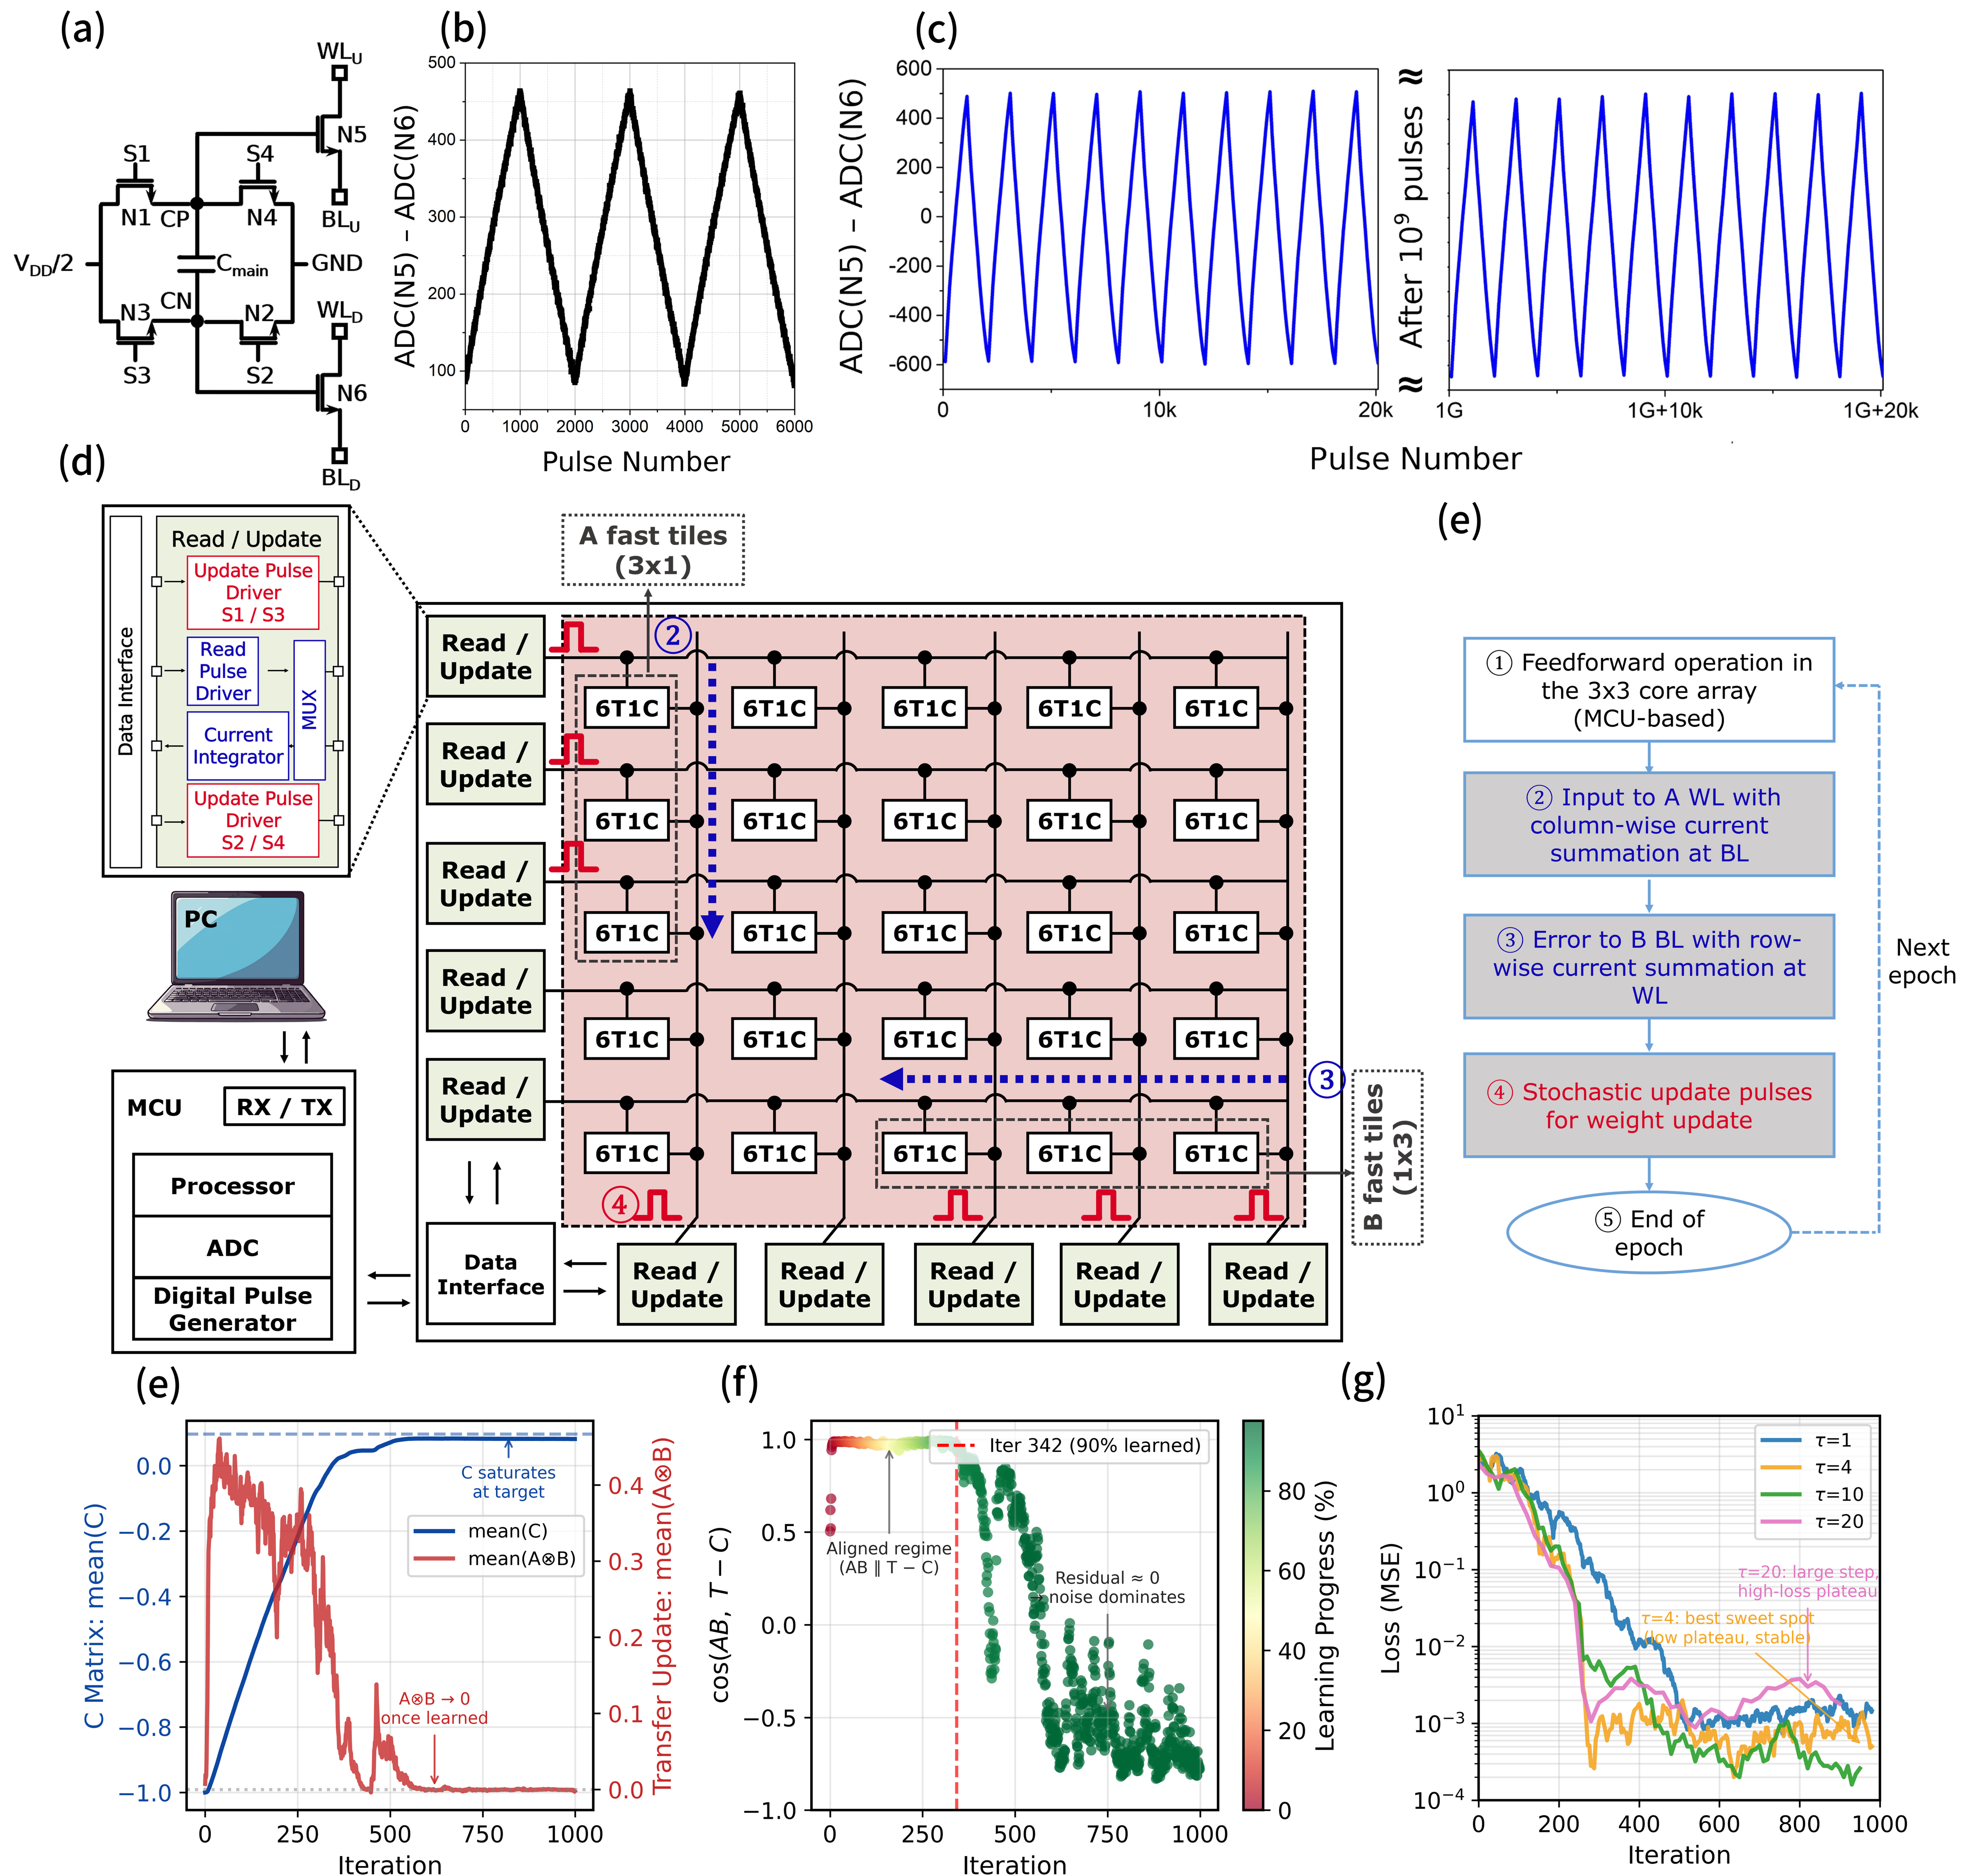
\includegraphics[width=\linewidth]{Figure3.png}
  \caption{\textbf{Experimental validation of 6T1C auxiliary tiles.} 
(a) Schematic of the 6T1C synaptic device. (b) Weight update characteristics of the 6T1C device, demonstrating ~1,000 multi-level states with high linearity and symmetry. (c) Endurance characteristics of the 6T1C device. (d) Hardware setup and synaptic array configuration for the regression task. (e) Experimental workflow of the regression task, where shaded regions indicate operations executed on the crossbar array. (f)–(h) Hardware-in-the-loop regression dynamics: core-weight, alignment, and MSE loss evolution.}
  \label{fig:main_fig3}
\end{figure*}

\begin{figure*}[t]
  \centering
  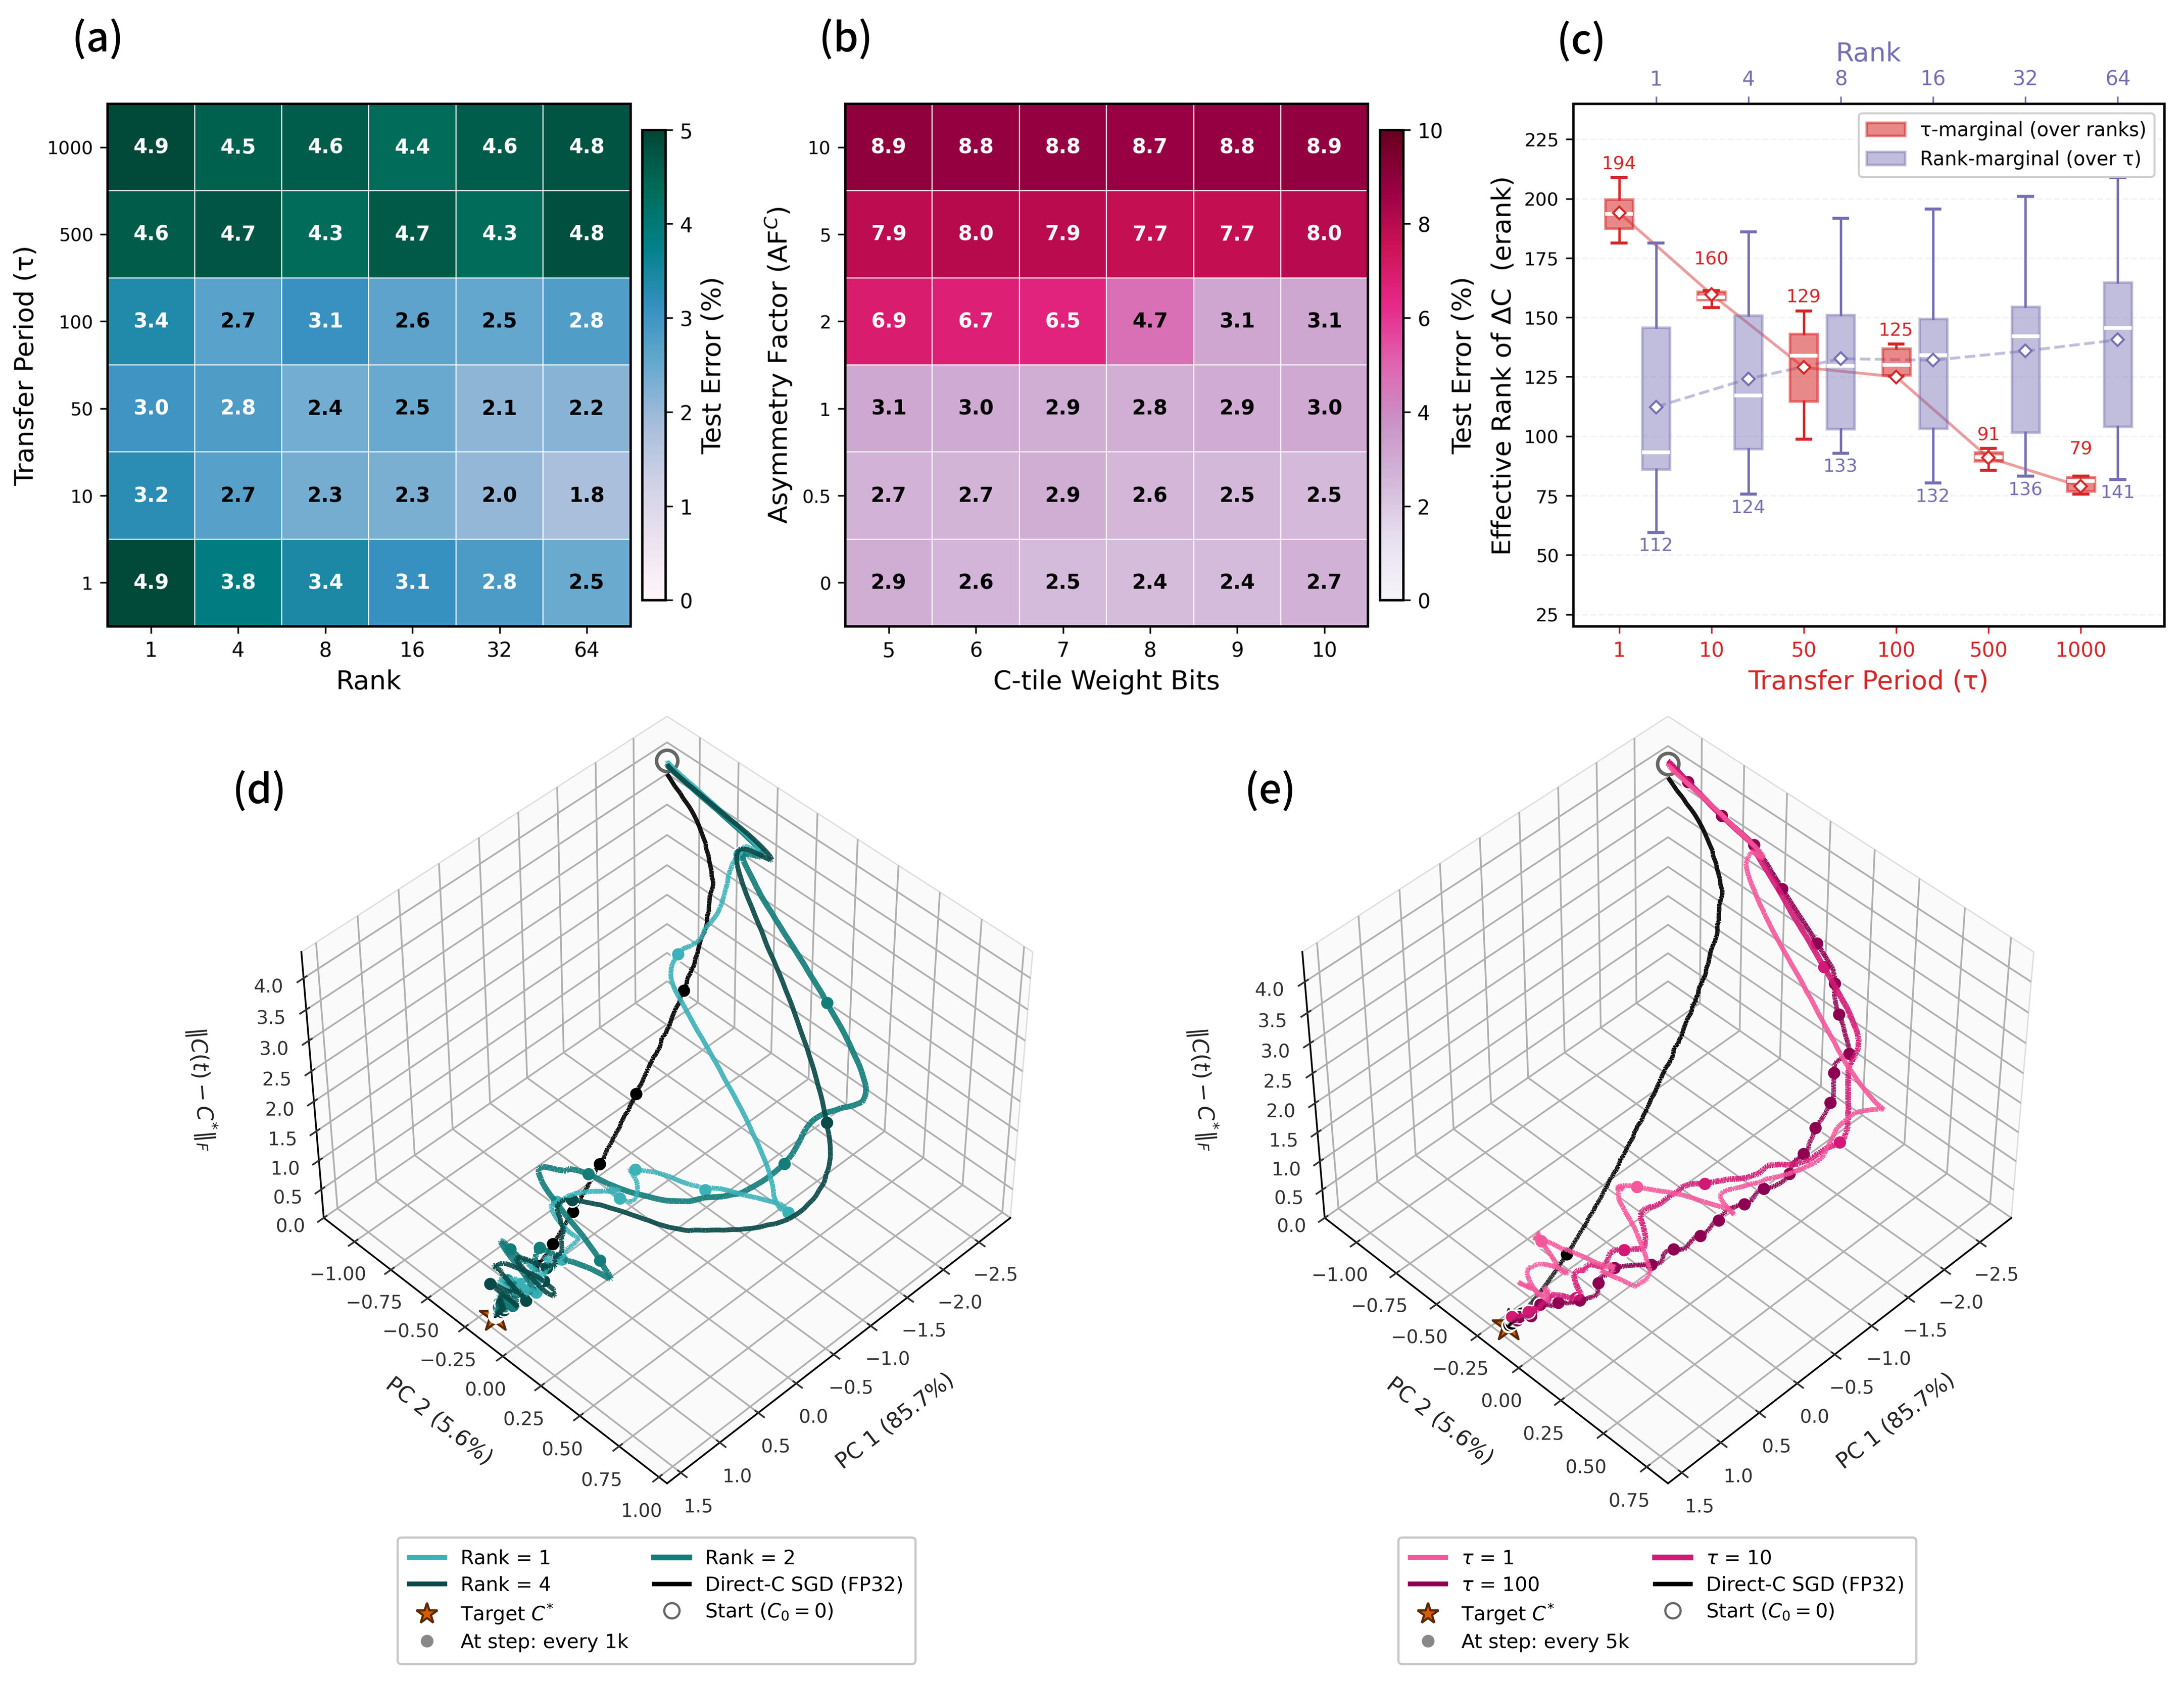
\includegraphics[width=0.92\textwidth]{Figure4.png}
  \caption{\textbf{Training trajectories and MNIST evaluation of LR-TT under on-chip scratch training.}
(a) Test-error heat map over low-rank dimension $r$ and transfer interval $\tau$, showing that test error decreases gradually as $r$ increases and is minimized near $\tau=10$ over most of the rank range, with the optimum shifting to larger $\tau$ only at the lowest ranks. (b) Test-error heat map over core-tile weight precision and core-tile asymmetry factor $\mathrm{AF}^{C}$ at fixed $r=8$ and $\tau=10$, showing that core-tile weight precision has only a modest effect in the low-$\mathrm{AF}^{C}$ regime, whereas test error rises sharply once $\mathrm{AF}^{C}>2$. (c) Box-plot statistics of the effective rank $\mathrm{erank}(\Delta C)$ of the core-tile increment measured at individual transfer events. The effective rank decreases strongly as $\tau$ increases, whereas it increases more gradually with $r$. 
(d) PCA-projected learning trajectories of the core matrix \(C\) in a controlled regression setting, with training loss on the \(z\)-axis, for fixed \(\tau=1\) and \(r\in\{1,2,4\}\) together with a direct-\(C\) SGD (FP32) baseline; diamond markers (\(\diamond\)) are placed every 1k steps to indicate convergence speed. As rank increases, the trajectory becomes smoother and more direct toward the target.
(e) Same projection for fixed \(r=1\) and \(\tau\in\{1,10,100\}\) with the same direct-\(C\) SGD (FP32) baseline; diamond markers (\(\diamond\)) are placed every 5k steps to indicate convergence speed. Smaller transfer periods produce more oscillatory trajectories, whereas larger transfer periods yield more direct but slower convergence.
}
  \label{fig:main_fig4}
\end{figure*}


\subsection{Hardware-in-the-loop low-rank learning with 6T1C auxiliary tiles}
\label{subsec:results_regression}

\noindent
We validate the hardware primitives required by LR-TT by implementing the low-rank auxiliary path on an oxide-semiconductor/capacitor-based 6T1C synaptic array and applying it to a controlled rank-1 hardware-in-the-loop regression task.
The 6T1C array was fabricated on an 8-inch wafer, and device measurements were carried out using a microcontroller unit (MCU) together with a discrete-device-based printed circuit board (PCB), following our prior setup; fabrication and measurement details are provided in the Methods.

\noindent\textbf{Synaptic update characteristics.}
Fig.~\ref{fig:main_fig3}a--c summarizes the device characteristics of the 6T1C synaptic primitive used for LR-TT auxiliary-state accumulation. The synaptic state is encoded as the capacitor voltage ($V_{\mathrm{cap}}$), and the cell employs dedicated transistor pairs for potentiation (N1, N2), depression (N3, N4), and readout (N5, N6). Because the programmed conductance is controlled by pulse width together with the TFT on-current, the device exhibits gradual bidirectional updates over an approximately $10^{3}$-level window while maintaining high linearity and near-symmetric response. Bias optimization further confirms scalability of the usable state window and retention compatible with the time scale of the present hardware-in-the-loop experiments (Supplementary Section~S1). Endurance measurements also indicate that the device can sustain the repeated rewriting required for an auxiliary tile during transformer-level adaptation \cite{ambrogio2018analogtraining,li2018insitu,legallo2018mixedprecision,mackin2022weightprogramming,won2023advs_6t1c,kang2025advs_disturbance}.

\noindent\textbf{Circuit-level operation.}
Fig.~\ref{fig:main_fig3}d--e presents the array configuration and hardware learning workflow. The 5$\times$5 array shows uniform update trajectories across all 25 cells (Supplementary Section~S1), after which a 1$\times$3 subarray and a 3$\times$1 subarray are assigned to the $A$ and $B$ factors, respectively. To isolate auxiliary-state accumulation from core-state non-idealities, the core matrix $C$ is maintained as MCU software variables. During each learning step, the forward response is first computed from $C$, and the resulting input and error signals are then converted into pulse-width-coded controls applied to the selected $A/B$ subarrays. Column-wise current summation in $A$ and chopper-assisted row-wise MAC readout in $B$ generate the projected signals required for factor-wise low-rank updates. These signals are digitized by the MCU and used to trigger fully parallel stochastic programming of the selected cells, using a previously developed disturbance-aware update scheme to mitigate write disturbance \cite{won2023advs_6t1c,kang2025advs_disturbance}. A photograph of the overall hardware setup for the demonstration is provided in Supplementary Section~S2.

\noindent\textbf{Rank-1 regression demonstration.}
We then demonstrate a closed hardware-in-the-loop LR-TT update cycle on a controlled rank-1 regression task.
Because the forward path is computed from the core state \(C\),
loss reduction occurs through discrete \(BA\!\rightarrow C\) transfer events.
Fig.~\ref{fig:main_fig3}f--h shows the resulting core-state trajectory, alignment with the target, and MSE loss evolution, confirming that the measured 6T1C \(A/B\) tiles can accumulate projected updates and transfer them to \(C\) under physical pulse programming.
Detailed core and auxiliary trajectories under different transfer periods are provided in Supplementary Section~S3.

\subsection{\texorpdfstring{Small-scale on-chip scratch training: task evaluation and trajectory analysis}{Small-scale on-chip scratch training: task evaluation and trajectory analysis}}
\label{subsec:results_scratch}

\noindent
We first evaluate LR-TT on MNIST classification \cite{lecun1998gradient} using an MLP, with the low-rank auxiliary state implemented on 6T1C arrays. We then complement the task-level results with a trajectory analysis on a controlled regression problem. Together, these small-scale experiments allow the accumulate--transfer dynamics of LR-TT to be examined before moving to transformer fine-tuning. As shown in Fig.~\ref{fig:main_fig4}, an appropriate choice of the transfer period $\tau$ stabilizes training across the full rank range, and even the rank-1 case can approach the performance regime of full training.

\noindent\textbf{Interplay of rank and transfer interval.}
Fig.~\ref{fig:main_fig4}a maps the MNIST test error over rank $r\in\{1,4,8,16,32,64\}$ and transfer interval $\tau\in\{1,10,50,100,500,1000\}$. Performance improves gradually with increasing $r$, but the stronger dependence is on $\tau$. Across most tested ranks, the minimum error occurs near $\tau=10$, and the best configuration reaches \(98.19\%\) accuracy at \(r=64\). The main result is therefore a clear optimum at an intermediate transfer interval. When $\tau$ is too small, transfer occurs before successive rank-limited updates have accumulated into a sufficiently informative correction. This interpretation is consistent with ReLoRA, where repeated low-rank updates require a finite accumulation window to build a richer overall change \cite{lialin2023relora}. When $\tau$ is too large, the opposite problem appears. The auxiliary state can accumulate useful history, but the core state is updated too infrequently for that information to influence learning effectively. This behavior is consistent with Tiki-Taka, where performance depends on how often the accumulated auxiliary-state update is transferred to the core weights \cite{gokmen2020tikitaka,lee2022tikitaka_asymmetry,rasch2024fastrobust}. By contrast, resetting \(B\) to its zero-reference state after each transfer lowers the accuracy relative to retaining \(B\) and shifts the optimum toward a longer transfer interval near \(\tau=100\) (see Supplementary Section~S5). This shift is consistent with the reset interrupting cross-window factor accumulation: \(B\) must be rebuilt from the retained \(A\) at the beginning of each accumulation window before coupled \(A/B\) adaptation can resume, thereby reducing the effectiveness of short transfer intervals.

\noindent\textbf{Sensitivity to core-tile non-idealities.}
Fig.~\ref{fig:main_fig4}b compares the effects of core-array weight resolution and core-array asymmetry by varying the nominal C-tile precision from 5 to 10 bits together with the asymmetry factor \(\mathrm{AF}^{C}\in\{0.0,0.5,1.0,2.0,5.0,10.0\}\). At \(\mathrm{AF}^{C}\leq 1\), the test error remains below about \(3.1\%\) across the full 5--10-bit range, indicating that this small MLP is relatively insensitive to moderate C-tile quantization. The stronger dependence is on asymmetry. At \(\mathrm{AF}^{C}=2\), increasing the C-tile precision partially recovers the performance, with 9--10 bits approaching the low-asymmetry regime. Once \(\mathrm{AF}^{C}\geq 5\), however, the error exceeds \(7.6\%\) almost independently of nominal bit resolution. The dominant limitation across these conditions is therefore asymmetric programming of the core tile rather than finite weight resolution.

\noindent
This trend is qualitatively consistent with the MNIST asymmetry analysis of Lee et al., which identified the most robust region around AF $\approx 1$ for both auxiliary and core arrays and showed that increasing main-array asymmetry makes the core-state update less frequent and more oscillatory \cite{lee2022tikitaka_asymmetry}. The stronger sensitivity observed here is plausibly related to the present LR-TT realization, in which the visible model is defined entirely by $C$. As a result, asymmetry in the core tile perturbs the forward path directly, and the low-rank state is written to $C$ through repeated rank-1 transfers without the digital filtering used in TTv2 to relax device-state requirements \cite{rasch2024fastrobust}. 

\noindent\textbf{Effective-rank growth in the core-state.}
Fig.~\ref{fig:main_fig4}c reports the statistics of \(\mathrm{erank}(\Delta C)\) for the cumulative core-state update, with the exact definition and evaluation procedure given in Supplementary Section~S5. Although each individual transfer is rank-limited by construction, repeated transfers progressively expand the update space of \(C\). The mean effective rank decreases monotonically with \(\tau\), from about 194 at \(\tau=1\) to about 79 at \(\tau=1000\), and increases more gradually with rank, from about 112 at \(r=1\) to about 141 at \(r=64\). LR-TT is therefore not confined to a permanently rank-\(r\) update at the core state. Instead, repeated low-rank transfers accumulate into a substantially richer modification of \(C\). At the same time, the largest \(\mathrm{erank}(\Delta C)\) is obtained at \(\tau=1\), whereas the best classification accuracy is obtained near \(\tau=10\). Effective-rank growth alone is therefore not sufficient to explain training quality. Fig.~\ref{fig:main_fig4}c therefore complements Fig.~\ref{fig:main_fig4}a by showing that the optimum near $\tau=10$ is not explained by effective-rank growth alone, but by the balance between enriching the cumulative core-state update and transferring it early enough to benefit learning. 

\noindent\textbf{Core-state trajectory analysis on simulated regression.}
To complement the preceding task-level results with a geometric view of the core-state optimization path, a \(9\times9\) regression problem was used in simulation. The learning trajectory of the visible core matrix \(C\) was visualized by applying PCA to the vectorized \(C\) weights \cite{lorch2016visualizing,li2018visualizing}, with the PCA basis fitted jointly over all trajectories shown in panels d and e. In this way, Fig.~\ref{fig:main_fig4}d,e complements the task-level trends in Fig.~\ref{fig:main_fig4}a and the cumulative-update statistics in Fig.~\ref{fig:main_fig4}c by showing how the visible core state evolves geometrically during learning.

As shown in Fig.~\ref{fig:main_fig4}d, the PCA trajectories at fixed \(\tau=1\) exhibit a clear dependence on the low-rank dimension. Each transfer event can modify \(C\) only through an update of rank at most \(r\), so smaller ranks restrict the number of update directions that can be combined within a single consolidation step, consistent with the low-rank parameterization of LoRA \cite{hu2021lora}. As \(r\) increases, the trajectory becomes smoother and more direct, and the step-milestone markers indicate faster progress toward the target. The direct-\(C\) SGD (FP32) baseline converges along the most direct path, serving as an unconstrained reference. Fig.~\ref{fig:main_fig4}d therefore shows that increasing rank improves both the convergence speed and the geometric regularity of the core-state optimization path.

Fig.~\ref{fig:main_fig4}e shows that the geometry of the learning trajectory also depends on the transfer period. At fixed \(r=1\) and \(\tau\in\{1,10,100\}\), smaller transfer periods produce broader and more oscillatory paths, indicating that the core state is corrected frequently before the auxiliary state has accumulated a sufficiently coherent correction. As \(\tau\) increases, each consolidation step moves \(C\) more directly toward the target, but the sparser step-milestone markers show that convergence becomes correspondingly slower. Fig.~\ref{fig:main_fig4}e therefore highlights a trade-off between transfer frequency and convergence speed, indicating that LR-TT requires an intermediate transfer period to balance directional efficiency with timely consolidation.

The sensitivity of the optimization trajectory to device nonlinearity is examined in Supplementary Fig.~S5, where the asymmetry factor is varied for both the core tile and auxiliary tiles.

%----------------------------------------------------
\begin{figure*}[t]
  \centering
  \begin{subfigure}{0.92\textwidth}
    \centering
    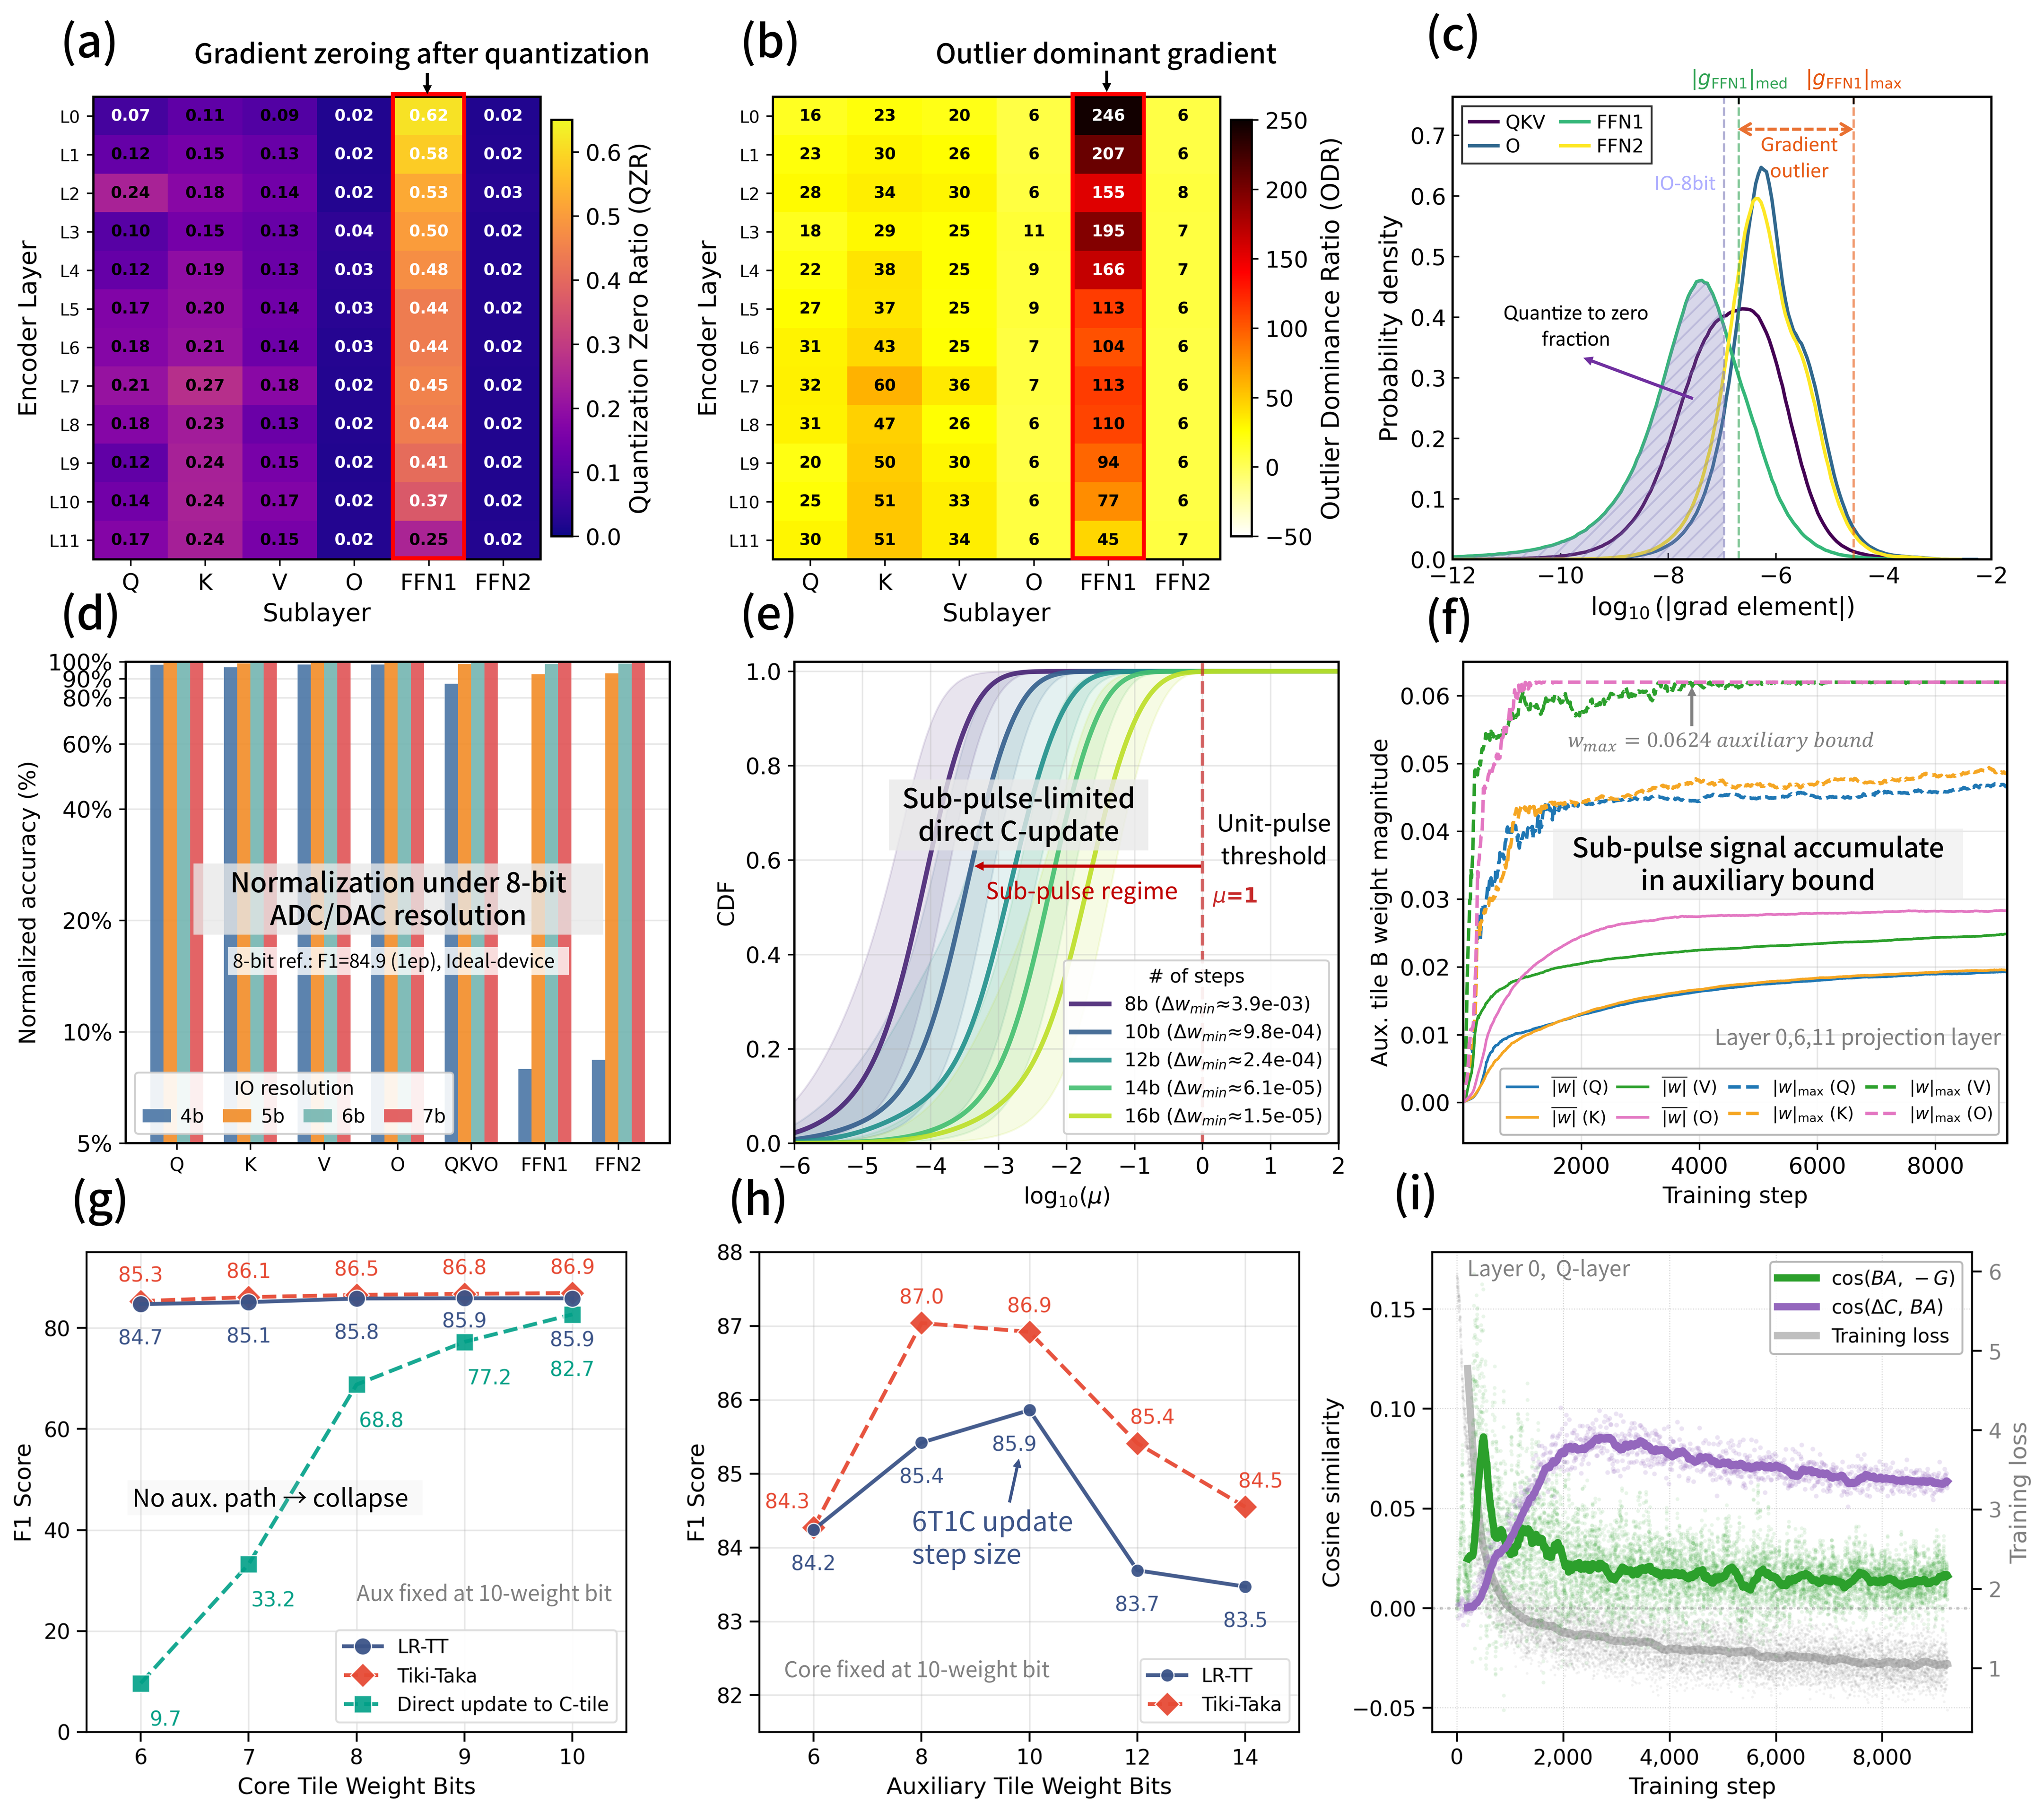
\includegraphics[width=\linewidth]{Figure5.png}
  \end{subfigure}
  \vspace{0.5em}
  \caption{\textbf{Transformer-level quantitative analysis of BERT-base fine-tuning on SQuAD v1.1.}
(a)--(c) Backward QZR and ODR heat maps and representative gradient distributions at 8-bit I/O resolution show that backward quantization damage is highly localized across layers and mapped sublayers, and is most severe in FFN1. Under limited I/O precision, a few large outliers compress the dynamic range available to low-magnitude gradient elements, so that a substantial fraction of nonzero gradient elements are quantized to zero.
(d) End-to-end sublayer-wise analysis identifies FFN1 as the most I/O-sensitive mapped sublayer, while isolated \(Q\), \(K\), \(V\), and \(O\) projections remain comparatively robust. Notably, the 4-bit collapse of FFN2 shows that end-to-end I/O sensitivity is not fully predicted by backward QZR/ODR severity alone.
(e) Update-path diagnostics show that, under this outlier-dominated backward regime, the cumulative distribution of elementwise expected pulse counts lies largely below the unit-pulse threshold. As a result, direct updates at low weight precision lose a large fraction of gradient information, and the realized update direction is only weakly aligned with the target gradient.
(f) Training-step evolution of the auxiliary \(B\) tile weight magnitudes (mean and maximum), averaged over Q/K/V/O sublayers across layers 0, 6, and 11, showing progressive weight growth within the programmable range.
(g) F1 as a function of core-tile precision at fixed auxiliary-tile conditions, comparing LR-TT, Tiki-Taka, and single-RPU direct update.
(h) F1 as a function of core-tile precision at fixed 10-bit core-tile resolution, comparing LR-TT and Tiki-Taka.
(i) Cosine similarity between the auxiliary-tile product and the negative gradient (\(\cos(BA, -G)\)) and between the actual core-tile update and the intended transfer (\(\cos(\Delta C, BA)\)), with training loss, for layer 0 attention query.}
\label{fig:main_fig5}


\end{figure*}

%----------------------------------------------------
%----------------------------------------------------
%===================================================
\begin{figure*}[t]
  \centering
  \begin{subfigure}{0.92\textwidth}
    \centering
    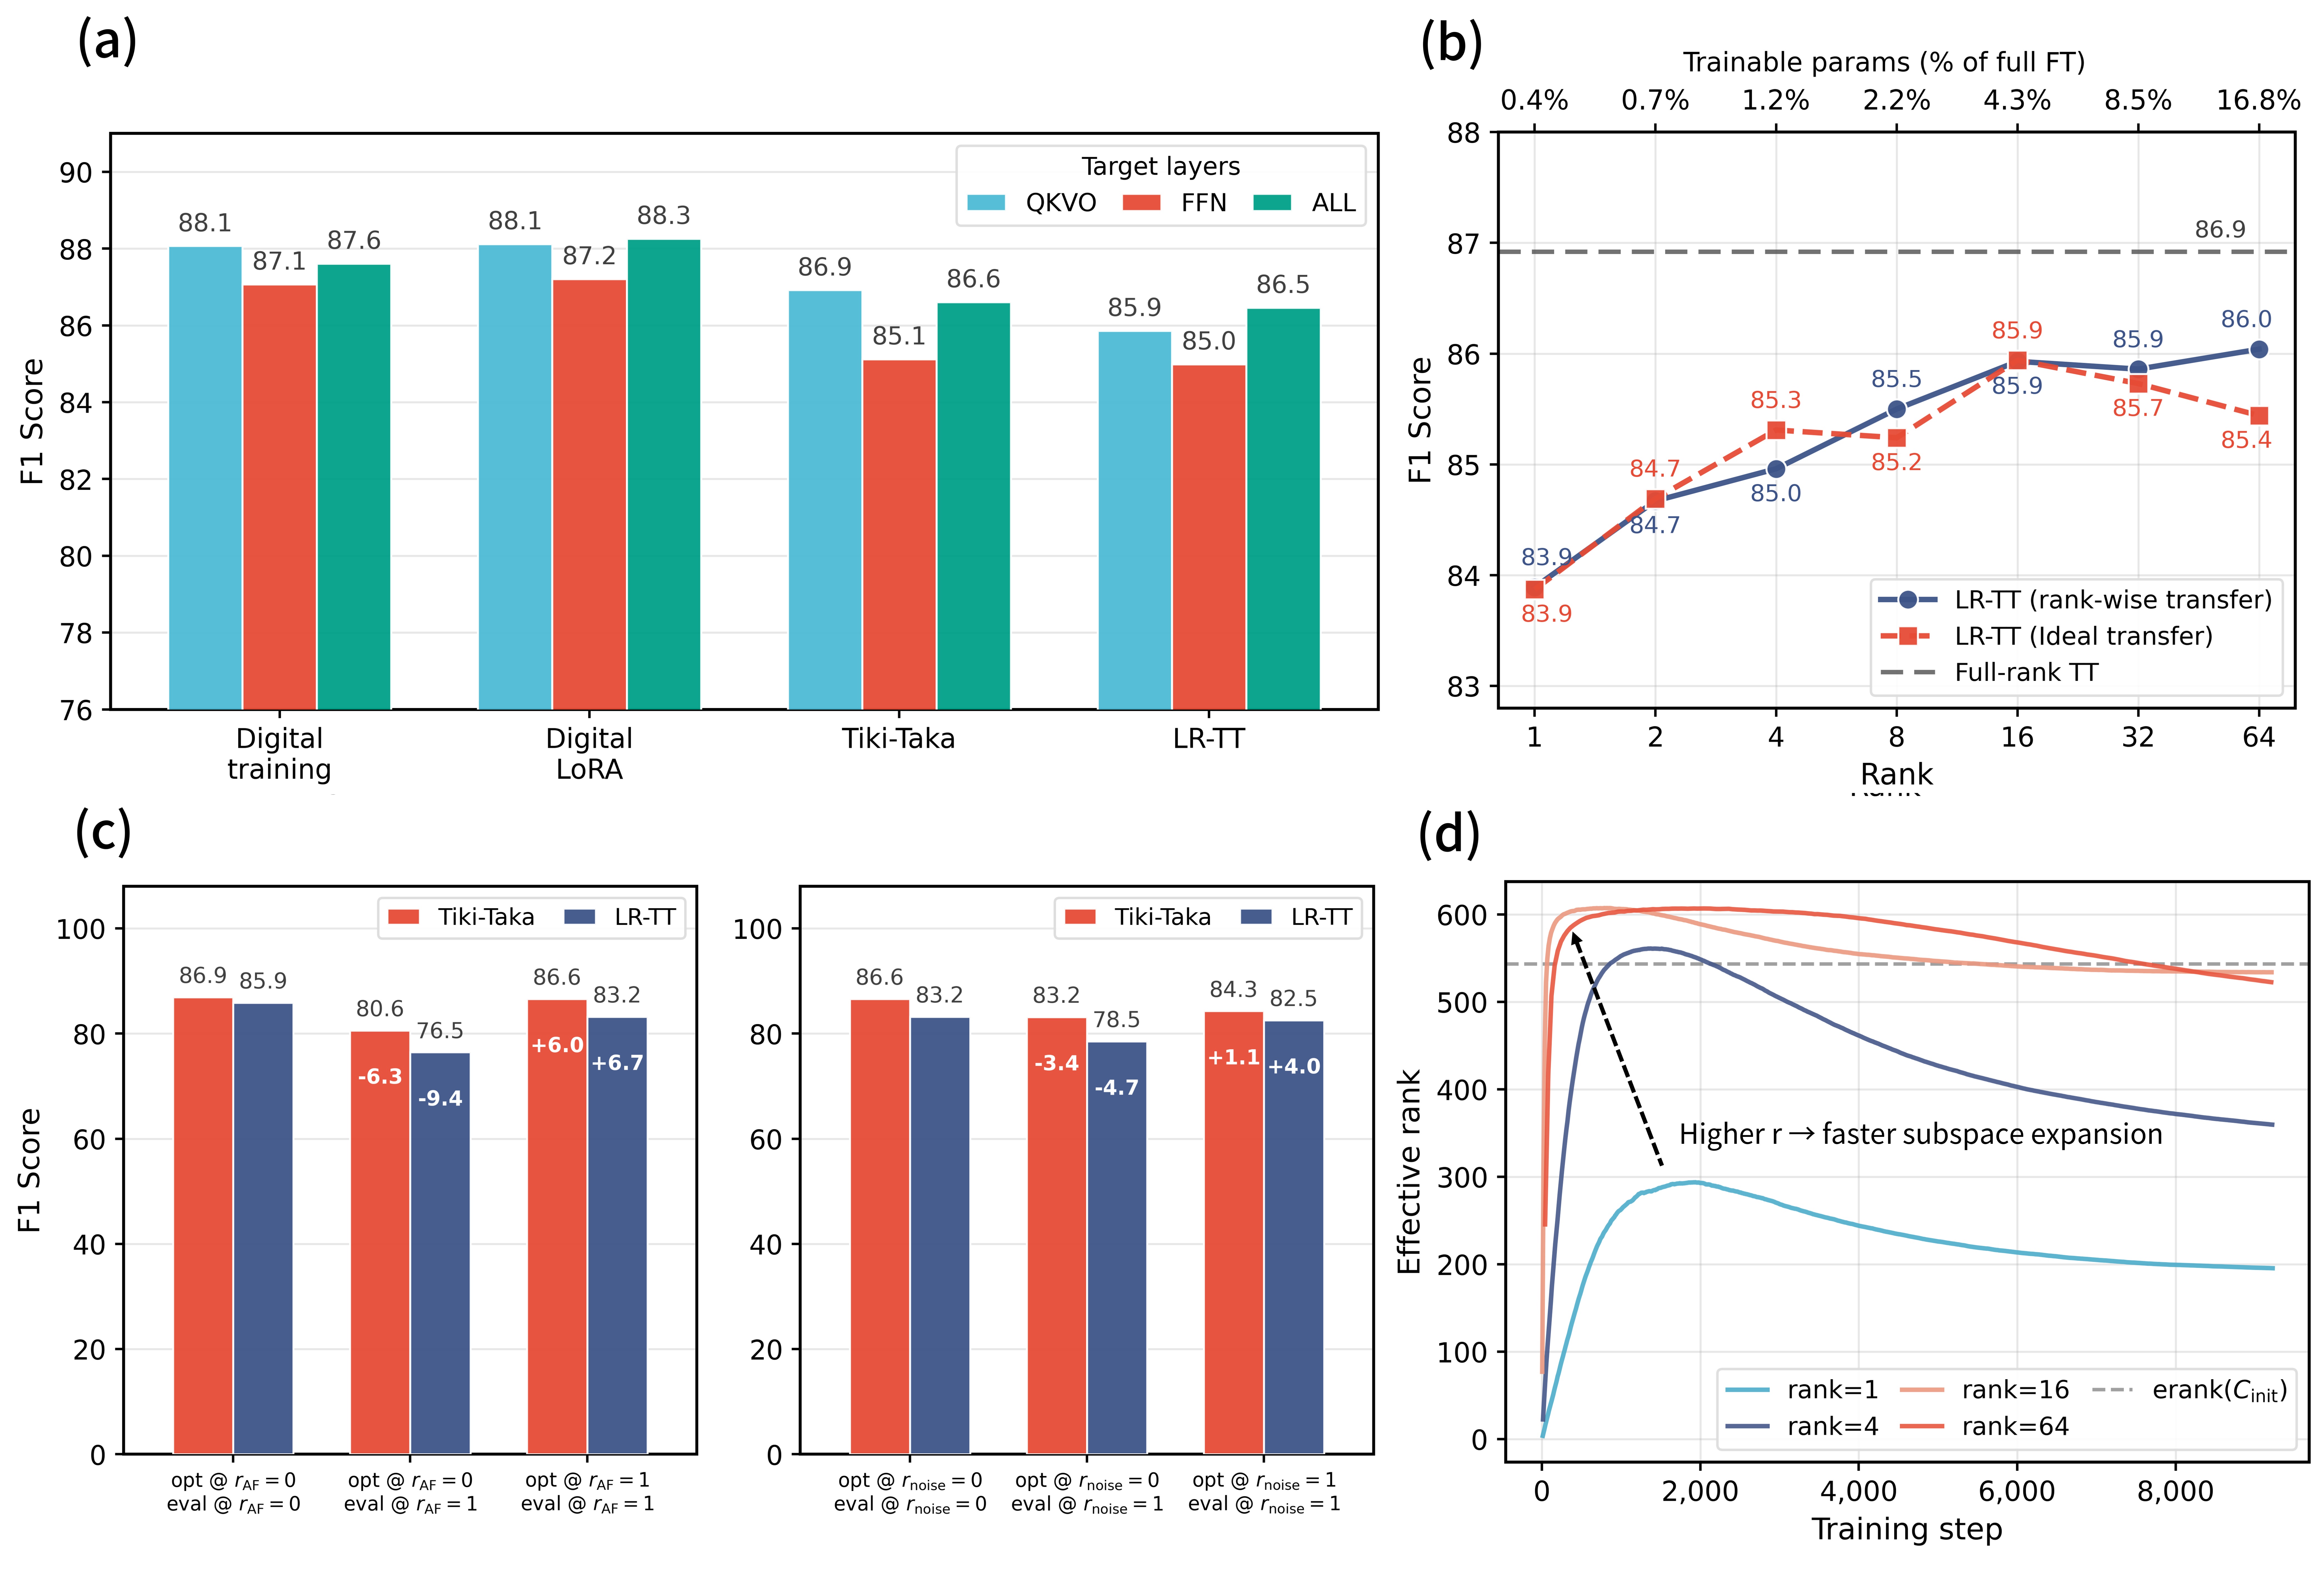
\includegraphics[width=\linewidth]{Figure6.png}
  \end{subfigure}
  \vspace{0.5em}

\caption{\textbf{Ablation and sensitivity analysis of LR-TT in BERT-base fine-tuning on SQuAD v1.1.}
(a) F1 comparison across mapped-layer configurations (QKVO, FFN, and ALL) for full digital fine-tuning, digital LoRA (\(r=32\)), full-dimensional Tiki-Taka, and LR-TT (\(r=32\)). The QKVO\(>\)FFN ordering is consistent across all four methods.
(b) F1 score as a function of rank for rank-wise stochastic transfer and ideal transfer under QKVO mapping, the latter reusing the per-rank hyperparameters optimized for rank-wise transfer without re-tuning; the trainable-parameter ratio (auxiliary \(A\)/\(B\) weights plus the shared digital parameters, relative to fully training all mapped projections; the core tile is updated only via transfer and is not counted) is shown on the upper axis. Performance saturates from \(r=16\) onward, and the small gap between the two transfer conditions indicates that stochastic pulse-transfer quantization does not substantially degrade end-to-end performance.
(c) Robustness to auxiliary-device non-idealities under QKVO mapping at \(r=32\). On each axis, a scale value of 1 corresponds to the nominal 6T1C characteristic and 0 to its idealized counterpart (symmetric updates for \(r_{\mathrm{AF}}\); zero noise/variation for \(r_{\mathrm{noise}}\)). Each panel compares three conditions along its non-ideality axis: hyperparameters tuned for the idealized level and evaluated there (\(\mathrm{opt@0,\,eval@0}\)), the same hyperparameters evaluated at the nominal 6T1C level without re-tuning (\(\mathrm{opt@0,\,eval@1}\)), and hyperparameters re-tuned at the 6T1C level (\(\mathrm{opt@1,\,eval@1}\)); white labels give the F1 change relative to the preceding condition (degradation and recovery, respectively).
Left: asymmetry-factor scale \(r_{\mathrm{AF}}\) at \(r_{\mathrm{noise}}=0\). Right: noise/variation scale \(r_{\mathrm{noise}}\) at fixed \(r_{\mathrm{AF}}=1\), i.e., on the asymmetric 6T1C device. The full dependence on \(r_{\mathrm{AF}}\) and \(r_{\mathrm{noise}}\) is provided in Supplementary Fig.~S8.
(d) Training-step evolution of the effective rank of the cumulative core-tile update \(\erank(\Delta C)\) (the deviation of the core weights from their pretrained values), for \(r\in\{1,4,16,64\}\) at the layer-0 query projection under the \(r_{\mathrm{AF}}=0\) condition; the dashed line marks the effective rank of the pretrained weight matrix itself. Although each individual transfer adds at most a rank-\(r\) update, the accumulated update attains an effective rank far above \(r\), at the highest ranks transiently exceeding that of the pretrained weights.}
  \label{fig:main_fig6}
\end{figure*}

\subsection{Transformer on-chip fine-tuning on BERT-base: algorithmic and system-level evaluation}
\label{subsec:results_transformer}


\noindent
We next consider transformer on-chip fine-tuning, where the dominant bottlenecks differ qualitatively from those in the preceding MNIST study. For BERT-base \cite{devlin2019bert} fine-tuning on SQuAD v1.1 \cite{rajpurkar2016squad}, the critical issues, as detailed in Fig.~\ref{fig:main_fig5}, are backward outliers, layer- and sublayer-dependent I/O precision sensitivity, and sub-pulse-limited updates under analog programming. Recent studies of quantized transformer training have shown that pretrained transformers can exhibit large weight, activation, and output-gradient outliers, making low-precision optimization particularly difficult \cite{ashkboos2025halo,bondarenko-etal-2021-understanding,xi2023training}. Consistent with this, quantized training more generally continues to rely on a higher-precision carry path, because many updates fall below the discretization gap of the reduced-precision representation \cite{nikdan2026eco}. In this background, we first diagnose the backward-gradient and update-path bottlenecks that make direct analog writing insufficient for transformer fine-tuning. We then characterize the training behavior of LR-TT under these conditions, including auxiliary-tile weight dynamics, tile precision requirements, gradient alignment, and the effective rank of the cumulative core-tile update. Finally, we evaluate the sensitivity of LR-TT to mapped-layer configuration, rank, and device non-idealities.

\noindent\textbf{Backward quantization damage and I/O sensitivity.}
Fig.~\ref{fig:main_fig5}a--c shows that backward quantization damage is highly non-uniform across layers and mapped sublayers; metric definitions for QZR, ODR, and the associated gradient-distribution analyses are given in the Methods. FFN1 is the dominant bottleneck, while \(O\) and FFN2 remain comparatively benign. Among the attention projections, \(K\) is the most affected, while \(Q\) and \(V\) are less severely degraded. The representative gradient distributions further indicate that the effective dynamic range is narrow: a few large elements set the quantization scale, whereas a substantial fraction of the low-magnitude body falls below the zero threshold and is quantized to zero. The remaining nonzero components are therefore distributed unevenly across vectors, so that many vectors retain only weak gradient signal after quantization. This pattern is most severe in FFN1, consistent with the role of FFN1 as the expansion projection before the GeLU nonlinearity, a position in which outlier-driven scaling is less well tolerated under limited I/O precision.

\noindent
Fig.~\ref{fig:main_fig5}d shows that these layerwise trends are largely reflected in the end-to-end F1 results. The main exception is FFN2: although its backward QZR/ODR is comparatively mild, its F1 score drops sharply at 4 bit. Because FFN2 sits at the output of the feed-forward branch, immediately before residual addition and layer normalization, quantization there perturbs the block output directly and is therefore less well tolerated.

\noindent\textbf{Sub-pulse regime and auxiliary-tile carry-path requirements.}
Fig.~\ref{fig:main_fig5}e diagnoses the update path directly. Across all examined layers and mapped sublayers, the effective pulse count remains deep in the sub-pulse regime, with median \(\mu\) typically between \(10^{-4}\) and \(10^{-3}\), so that essentially all elementwise updates satisfy \(\mu < 1\). This sub-pulse bottleneck follows from the outlier-dominated backward-gradient structure diagnosed above. Under stochastic pulsed outer-product updates with dynamic pulse-length management and vector-wise scaling \cite{rasch2021aihwkit,legallo2023aihwkit}, a few large gradient entries set the scale within each update vector, so that most elementwise update signals remain below the unit-pulse threshold. A similar problem has been reported in digital low-precision training, where small updates are lost under direct low-precision writes and are resolved through an auxiliary carry path \cite{nikdan2026eco}. On AIMC hardware, the corresponding AIMC solution is a Tiki-Taka-like auxiliary accumulation state that retains these sub-threshold corrections until they are transferred reliably to the core state. 

\noindent
Fig.~\ref{fig:main_fig5}f shows the training-step evolution of the auxiliary \(B\) tile weight magnitudes, averaged over the Q/K/V/O sublayers across layers 0, 6, and 11. The tile starts from near-zero initialization and grows progressively during training as sub-pulse updates accumulate over successive steps, confirming that the auxiliary carry path retains gradient information that would otherwise be lost under direct low-bit writing. The per-cell maximum saturates at \(|w|_{\max}^{A,B}\), while the mean absolute weight remains well below the bound. Because repeated stochastic pulse updates tend to diffuse weight magnitudes outward, this bounded behavior requires either a hard bound through a constrained \(|w|_{\max}^{A,B}\) or a soft bound through state-dependent update asymmetry; the interaction between these two mechanisms is further analyzed in Fig.~\ref{fig:main_fig6}c and Supplementary Fig.~S9. Supplementary Fig.~S7 shows the corresponding individual-cell weight trajectories for the \(A\), \(B\), and \(C\) tiles, where the core tile \(C\) retains its pretrained weight structure with only small perturbations from transfer updates.

\noindent
\textbf{Auxiliary and core tile precision requirements.}
Fig.~\ref{fig:main_fig5}g shows F1 as a function of core-tile precision at fixed auxiliary-tile conditions, comparing LR-TT against a single-RPU direct-update baseline and a full-dimensional Tiki-Taka baseline. LR-TT retains F1\(>\)84 even at 6-bit core-tile resolution, whereas the single-RPU baseline collapses to F1\(\approx\)10 at the same precision. Tiki-Taka maintains consistently higher F1 across the precision range owing to its full-dimensional auxiliary state. Fig.~\ref{fig:main_fig5}h shows the complementary per-bit-optimized dependence on auxiliary-tile precision at fixed 10-bit core-tile resolution, together with a full-dimensional Tiki-Taka baseline at matched bit conditions. LR-TT peaks at 10-bit auxiliary precision (F1 85.9) and stays above F1 83.4 across the 6--14-bit range, while Tiki-Taka remains higher throughout owing to its full-dimensional auxiliary state. The gap between the two is widest at intermediate bit counts (1.7 F1 at 12-bit) and closes almost completely at 6-bit (0.03 F1), where the coarse auxiliary resolution rather than low-rank compression sets the limit for both methods. These results demonstrate that the core tile tolerates substantially coarser quantization than the auxiliary tile, consistent with the core tile receiving only periodic transferred updates rather than continuous sub-pulse accumulation.

\noindent
\textbf{Transfer fidelity and gradient alignment.}
Fig.~\ref{fig:main_fig5}i evaluates the rank-wise stochastic transfer mechanism for a representative layer (layer 0, query projection). The cosine similarity \(\cos(\Delta C, 
BA)\) between the actual core-tile update and the intended transfer signal measures how faithfully the stochastic pulse transfer reproduces the accumulated auxiliary product. This quantity remains substantially below unity throughout training, reflecting the quantization gap inherent in finite-precision pulse programming on the core tile. The auxiliary-tile product also maintains a persistent, albeit noisy, alignment with the descent direction, as indicated by the positive moving average of \(\cos(BA, -G)\). This loose per-step alignment is consistent with the indirect optimization trajectories observed in the regression analysis (Fig.~\ref{fig:main_fig4}d,e), where LR-TT follows a more oscillatory path than direct-\(C\) SGD. Despite this, repeated transfers progressively build a rich cumulative update on the core tile, as confirmed by the effective-rank analysis in Fig.~\ref{fig:main_fig6}d. Supplementary Fig.~S10 shows the same analysis for layer 11 (attention output).

\noindent
\textbf{Mapped-layer comparison and rank scaling.}
Fig.~\ref{fig:main_fig6}a compares LR-TT fine-tuning performance across three mapped-layer configurations: Q/K/V/O attention projections only, FFN layers only, and all mapped layers, together with full digital fine-tuning, digital LoRA, and full-dimensional Tiki-Taka baselines. Among the LR-TT configurations, all-layer mapping achieves the highest F1 (86.5), followed by QKVO-only (85.9) and FFN-only (85.0). The same QKVO\(>\)FFN ordering is observed across all four methods, suggesting that attention projections contribute more to task adaptation than FFN layers for this task. Tiki-Taka reaches 86.9 (QKVO) and 86.6 (ALL), narrowing the gap to the digital baselines (88.1 and 88.3 for digital LoRA); unlike LR-TT it does not gain from all-layer mapping, indicating that the benefit of mapping more layers is specific to the low-rank auxiliary path. The remaining gap between LR-TT and Tiki-Taka reflects the cost of low-rank compression in the auxiliary path, while the gap between Tiki-Taka and digital LoRA is attributable to analog non-idealities. Fig.~\ref{fig:main_fig6}b shows the rank dependence of F1 for rank-wise stochastic transfer and ideal transfer, together with the trainable parameter ratio relative to full fine-tuning. For the ideal-transfer condition, the hyperparameters optimized under rank-wise transfer were reused without re-tuning. Both transfer methods show F1 increasing with rank up to saturation near rank 16, and the F1 gap between the two remains small across the rank range. This small gap indicates that the quantization loss inherent in rank-wise stochastic pulse transfer does not substantially degrade end-to-end performance, consistent with the transfer-fidelity analysis in Fig.~\ref{fig:main_fig5}i. At rank 1, LR-TT achieves F1\(>\)83 using only 0.4\% of the full fine-tuning trainable parameters, demonstrating that the cumulative transfer mechanism enables effective adaptation even at extreme parameter compression.

\begin{figure*}[t]
  \centering
  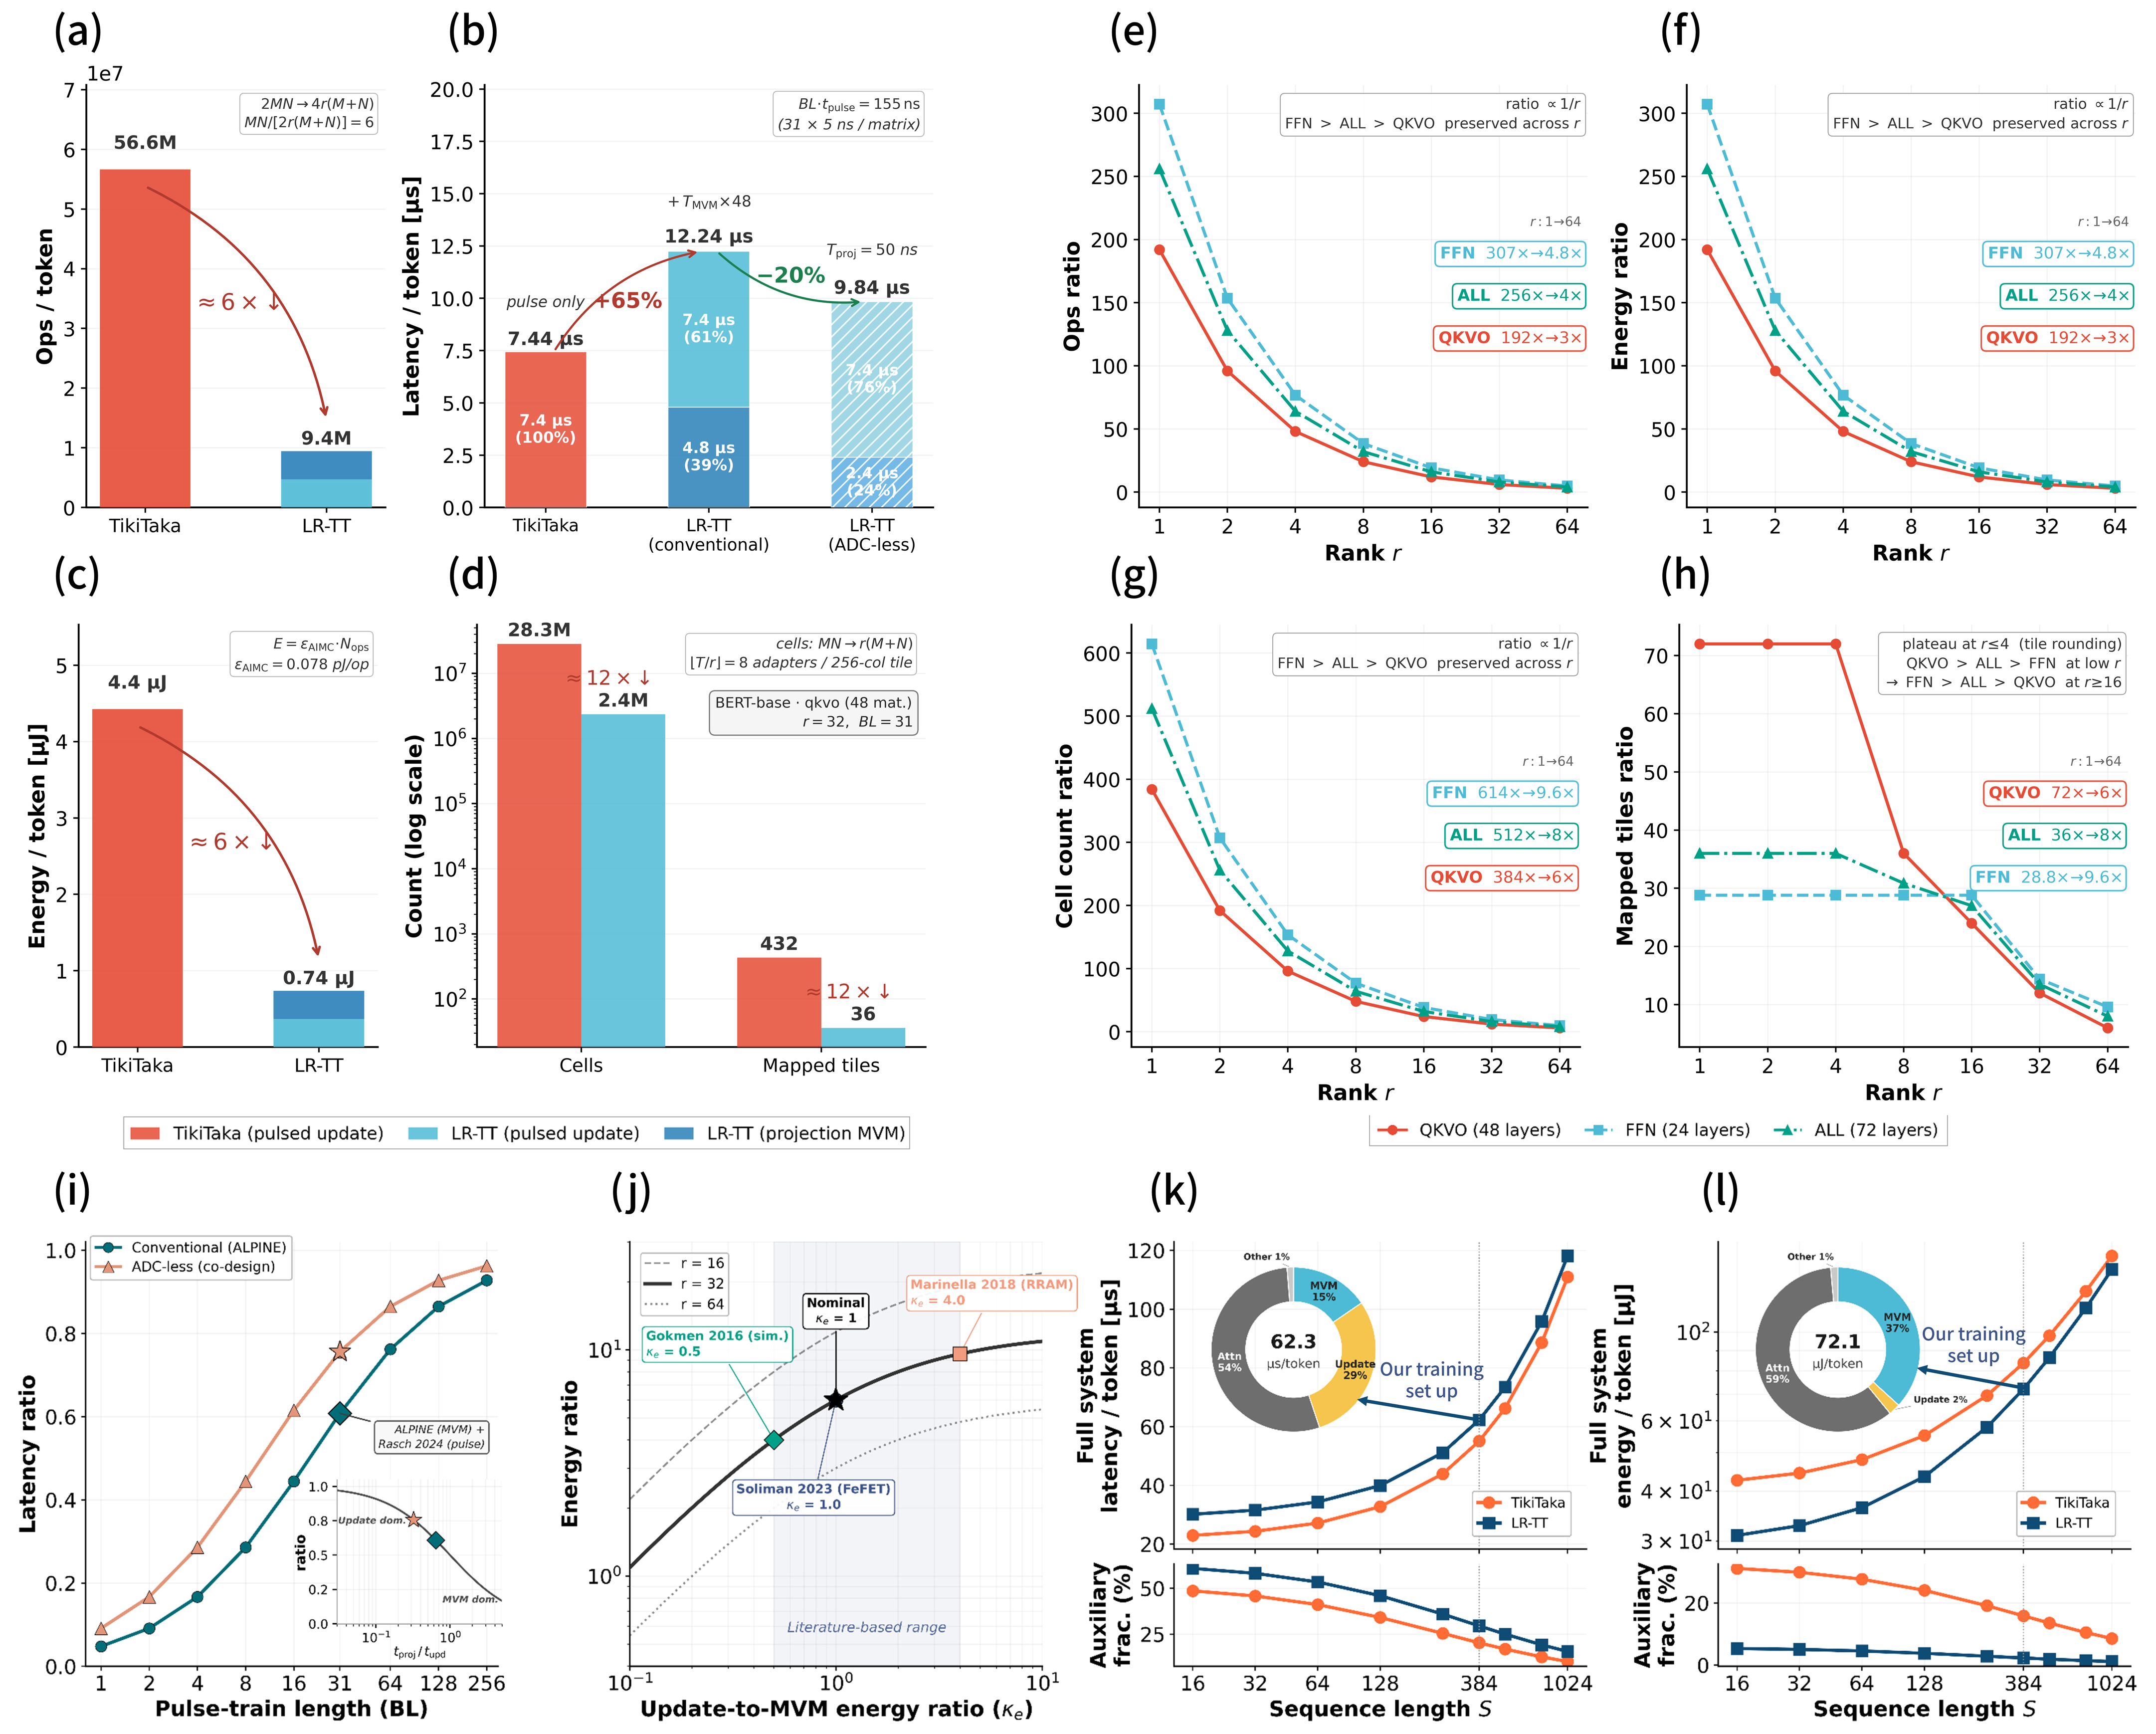
\includegraphics[width=0.98\textwidth]{Figure7.png}
\caption{\textbf{System-level latency, energy, and storage-efficiency analysis of LR-TT and Tiki-Taka in AIMC-mapped BERT-base fine-tuning.}
(a)--(d) summarize the Q/K/V/O-projection-only setting at \(r=32\). LR-TT strongly reduces the auxiliary-path operation count, energy, trainable cell count, and required tile count relative to TT, whereas the latency benefit remains more limited because the low-rank projection path introduces explicit readout overhead.
(e)--(h) report the reduction ratios in operation count, energy, trainable cell count, and required tile count versus rank for Q/K/V/O-projection-only, FFN-only, and all-layer mapping. Across all four metrics, the reduction decreases monotonically with rank and is most pronounced for FFN-only mapping.
(i) and (j) show the sensitivity of the latency ratio and energy ratio to pulse-train length and update-to-MVM energy ratio, respectively, for the same Q/K/V/O-projection-only setting.
(k) and (l) report the corresponding full-system latency and energy when the core path and digital transformer operations are included.}
  \label{fig:e2e_lrtt_tt}
\end{figure*}

\noindent
\textbf{Sensitivity to device non-idealities.}
Fig.~\ref{fig:main_fig6}c examines the robustness of LR-TT and full-dimensional Tiki-Taka to auxiliary-device update asymmetry and noise/variation, comparing for each non-ideality the benign optimum, the same hyperparameters at the degraded setting, and hyperparameters re-optimized at the degraded setting.
The right panel evaluates noise/variation robustness at fixed asymmetry-factor scale \(r_{\mathrm{AF}}=1\), corresponding to the nominal 6T1C-calibrated update-response asymmetry.
Without re-tuning, the \(r_{\mathrm{noise}}=0\)-optimized LR-TT condition drops from F1\(=83.2\) to 78.5 at \(r_{\mathrm{noise}}=1\), falls to F1\(\approx\)53 at \(r_{\mathrm{noise}}=2\), and collapses below F1\(=10\) at \(r_{\mathrm{noise}}=3\), whereas re-optimization at \(r_{\mathrm{noise}}=1\) restores F1\(=82.5\), maintains F1\(\approx\)82 across the 0--1 range, retains F1\(=71.4\) at \(r_{\mathrm{noise}}=3\), and collapses only at \(r_{\mathrm{noise}}=5\) (Supplementary Fig.~S8).
Re-optimization at the target noise/variation level thus moves the collapse threshold from \(r_{\mathrm{noise}}=3\) to 5 at the cost of less than 1 F1 point in the low-non-ideality regime; notably, LR-TT re-optimizes almost completely (82.5 vs.\ its benign optimum of 83.2), whereas Tiki-Taka retains a 2.3-point gap (84.3 vs.\ 86.6).
Notably, in contrast to the asymmetry-factor axis in the left panel, where the re-optimized condition fails at \(r_{\mathrm{AF}}=0\) because the device relies on the resulting soft-bound response, noise/variation scaling is reversible: the \(r_{\mathrm{noise}}=1\)-optimized condition functions normally at \(r_{\mathrm{noise}}=0\) because reducing stochastic and device-to-device variation does not violate any device-level operating assumption.
The left panel evaluates asymmetry robustness at \(r_{\mathrm{noise}}=0\): the \(r_{\mathrm{AF}}=0\)-optimized LR-TT condition (\(|w|_{\max}^{A,B}=0.063\), 10-bit auxiliary tile) achieves F1\(=85.9\) at zero asymmetry but drops to 76.5 at \(r_{\mathrm{AF}}=1\), and re-optimization there restores F1\(=83.2\) by moving to a substantially larger auxiliary bound (\(|w|_{\max}^{A,B}=1.0\)); the re-optimized condition fails at \(r_{\mathrm{AF}}=0\) (F1\(<\)10) because at this larger bound the device relies on the asymmetry-induced soft-bound response to prevent weight divergence, while already at \(r_{\mathrm{AF}}=0.5\) the half-strength asymmetry suffices to stabilize it (Supplementary Fig.~S8).
This complementary behavior indicates that the optimal operating regime depends on whether the auxiliary device provides an intrinsic soft-bound response through update asymmetry or relies on a constrained weight range; Tiki-Taka, by contrast, absorbs the nominal asymmetry with a smaller un-retuned drop (\(-6.3\) vs.\ \(-9.4\) F1) and re-optimizes essentially back to its benign optimum (86.6 vs.\ 86.9).
Together, these asymmetry-factor and noise/variation analyses emphasize that there is no universally optimal hyperparameter set: hyperparameters should be tuned at the deployment device's actual operating point---its native asymmetry-factor scale and noise/variation level---to obtain the most robust LR-TT performance on hardware.
Supplementary Section~S8 outlines a practical heuristic for selecting LR-TT hyperparameters from device-level asymmetry-factor and noise/variation specifications.
The \(r_{\mathrm{AF}}\)--\(|w|_{\max}^{A,B}\) interaction is further characterized in Supplementary Fig.~S9.

\noindent
\textbf{Effective rank of the cumulative core-tile update.}
Fig.~\ref{fig:main_fig6}d shows the training-step evolution of \(\erank(\Delta C)\) for different LR-TT ranks, where \(\Delta C = C_{\ell,t}-C_{\ell,0}\) is the cumulative deviation of the core weights from their pretrained values (Supplementary Section~S5). Despite each transfer event being rank-limited, the cumulative core-tile update achieves effective ranks far exceeding the nominal rank: at rank 1, \(\erank(\Delta C)\) peaks near 300, and at rank 64 it transiently exceeds the effective rank of the pretrained weight itself (\(\approx\)543, dashed line). The subsequent decline in \(\erank(\Delta C)\) during later training is consistent with convergence to a task-specific subspace, where successive transfers reinforce existing dominant singular directions rather than introducing new ones. This confirms that LR-TT is not confined to a permanently low-rank modification of the core matrix; instead, the repeated accumulate-and-transfer cycle progressively enriches the subspace of the cumulative update. This behavior is analogous to the cumulative rank growth observed in ReLoRA, where repeated low-rank merges build an effective update whose rank exceeds that of any single adapter \cite{lialin2023relora}. Higher nominal rank accelerates this enrichment by contributing more directions per transfer event, consistent with the monotonic F1 improvement observed in Fig.~\ref{fig:main_fig6}b.


\subsection{End-to-end system-level evaluation}
\label{subsec:PPA_transformer}

\noindent
We next compare LR-TT and the Tiki-Taka (TT) baseline at the system level using an analytical model calibrated to the ALPINE AIMC tile \cite{klein2023alpine}. The model is instantiated on the same AIMC-mapped BERT-base fine-tuning workload considered above, and the auxiliary-path cost is estimated following prior AIMC training studies on pulsed outer-product updates and periodic transfer to the core state \cite{gokmen2016rpu,gokmen2020tikitaka,gokmen2021ttv2,rasch2024fastrobust}. Fig.~\ref{fig:e2e_lrtt_tt} summarizes the auxiliary-path cost and its scaling in panels (a)--(j). Panels (i) and (j) remain in the Q/K/V/O-only auxiliary-path setting, whereas panels (k) and (l) extend the analysis to the full-system latency and energy after including the core path, digital attention, and other digital operations. Detailed modeling assumptions, mapped operators, and metric definitions are given in the Methods.

\noindent\textbf{Auxiliary-path efficiency and rank dependence.}
Fig.~\ref{fig:e2e_lrtt_tt}a--d summarizes the nominal Q/K/V/O-only auxiliary-path operating point at \(r=32\) (see Methods). Relative to TT, LR-TT reduces the auxiliary-path operation count from 56.6M to 9.4M per token and the corresponding energy from 4.4 to 0.74~\(\mu\)J per token. The trainable cell count decreases from 28.3M to 2.4M, and the required tile count decreases from 432 to 36. These reductions follow directly from the change in auxiliary-state scaling, since the TT auxiliary state scales with \(MN\), whereas the LR-TT auxiliary state scales with \(r(M+N)\). At the same operating point, conventional LR-TT reaches 12.24~\(\mu\)s per token rather than the 7.44~\(\mu\)s of TT because the low-rank projection path introduces an explicit readout overhead; the ADC-less co-design reduces this value to 9.84~\(\mu\)s per token.

\noindent
Fig.~\ref{fig:e2e_lrtt_tt}e--h extends the auxiliary-path comparison across rank for Q/K/V/O-only, FFN-only, and all-layer mapping, and reports the corresponding TT/LR-TT ratios in operation count, energy, trainable cell count, and required tile count. The largest savings are obtained in the low-rank regime, where the auxiliary state remains strongly compressed; as \(r\) increases, these benefits taper because the LR-TT auxiliary state scales with \(r(M+N)\). The strongest reduction appears in the FFN-only case, where the wider \(3072\times768\) and \(768\times3072\) matrices further amplify the gap between the full-dimensional and low-rank auxiliary states.

\noindent\textbf{Sensitivity to pulse length and update-energy assumptions.}
Fig.~\ref{fig:e2e_lrtt_tt}i isolates the LR-TT auxiliary update micro-cycle in the Q/K/V/O-only auxiliary path and examines how its pulse-write fraction varies with the pulse-train length \(BL\). The quantity of interest is \(t_{\mathrm{upd}}/(t_{\mathrm{proj}}+t_{\mathrm{upd}})\), which increases with \(BL\) because the relative contribution of projection readout decreases; at the nominal \(BL=31\), it is 0.608 for conventional projection readout and 0.756 for the ADC-less co-design. Fig.~\ref{fig:e2e_lrtt_tt}j evaluates the auxiliary-path energy robustness of LR-TT relative to TT as the update-to-MVM energy ratio \(\kappa_e\) is varied, showing that the LR-TT energy advantage persists across the examined \(\kappa_e\) range. The corresponding definitions and the literature basis of the \(\kappa_e\) range are given in the Methods.

\noindent\textbf{System-level sequence-length dependence.}
Fig.~\ref{fig:e2e_lrtt_tt}k,l extend the analysis to the all-layer full-system setting by including the core path and the common digital transformer operations. At the nominal operating point (\(S=384\), \(r=32\), \(BL=31\)), LR-TT yields a total latency of 62.29~\(\mu\)s per token, compared with 55.09~\(\mu\)s per token for TT. The corresponding LR-TT latency composition is 15.4\% core MVM, 29.5\% auxiliary path, 53.8\% digital attention, and 1.3\% other digital operations, while the energy composition at the same operating point is dominated by digital attention (59.5\%) and core MVM (36.8\%), with the auxiliary path contributing only 2.3\% and the remaining 1.4\% coming from other digital operations. Thus, LR-TT introduces a modest latency overhead through the explicit projection path while preserving a compact auxiliary energy budget. As the sequence length \(S\) increases, the shared sequence-length-dependent cost grows for both methods, so the auxiliary-path fraction decreases and the full-system latency and energy curves progressively converge, reflecting the increasing dominance of digital attention in the total system cost.

\section{Discussion}
\label{sec:discussion}

\noindent
In this work, we introduced Low-Rank Tiki-Taka (LR-TT), a core--auxiliary analog training scheme that makes Tiki-Taka-style in-situ learning compatible with parameter-efficient transformer adaptation \cite{hu2021lora,gokmen2020tikitaka,gokmen2021ttv2}. By replacing the full-size auxiliary matrix of Tiki-Taka with low-rank \(A/B\) auxiliary tiles, the method preserves the accumulate-and-transfer mechanism required for robust analog updates while changing the auxiliary-state scaling from \(MN\) to \(r(M+N)\). This distinction is important for transformer fine-tuning, where large dense projections dominate the mapped hardware footprint and many useful update components fall below the unit-pulse threshold of direct low-bit pulsed analog writing. The proposed scheme was evaluated across device, algorithm, task, and system levels. Measured IGZO-TFT/capacitor 6T1C arrays provided gradual and near-symmetric bidirectional updates suitable for the repeatedly written auxiliary path, and hardware-in-the-loop regression confirmed that measured \(A/B\) tiles can accumulate projected low-rank updates and transfer them to a forward-visible core state. MNIST training and controlled trajectory analyses further showed that repeated rank-limited transfers can build a richer cumulative update than a permanently rank-\(r\) modification of the core matrix. At the transformer scale, device-calibrated BERT-base fine-tuning evaluations on SQuAD v1.1 identified backward outliers, layer-dependent I/O sensitivity, and sub-pulse-limited updates as dominant obstacles to AIMC-based training. By retaining a high-resolution auxiliary accumulation path before transfer to the core state, the proposed design maintains task performance close to full-size-auxiliary Tiki-Taka as rank increases while substantially reducing auxiliary-path operation count, energy, trainable cells, and tile footprint. To our knowledge, this represents one of the first device-calibrated AIMC studies to evaluate a pulsed analog auxiliary update path for BERT-base-scale transformer fine-tuning.

\noindent
These results suggest that low-rank structure is most useful for AIMC training when it compresses the analog accumulation path rather than merely reducing the number of trainable software parameters. This distinguishes the approach from digital LoRA-adapter schemes for AIMC, in which low-rank modules reduce software training cost but remain outside the analog pulsed update loop \cite{li2026ahwa_lora}. Here, the low-rank factors themselves constitute the analog auxiliary accumulation state, so the compression acts directly on the physical update path. The same compression that reduces auxiliary cell count also concentrates write activity onto fewer auxiliary cells. The device requirement is therefore shifted from supporting a large full-size auxiliary matrix toward supporting compact, frequently written auxiliary tiles with high cycling endurance, near-symmetric bidirectional updates, and retention over the transfer window \cite{rasch2024fastrobust,won2023advs_6t1c}.

\noindent
The present implementation still relies on a hybrid analog--digital partition, calibrated system-level modeling, and explicit low-rank projection readout. The projection path introduces a modest latency overhead relative to full-size-auxiliary Tiki-Taka in the evaluated full-system setting, but this overhead is not the dominant system-level cost at the nominal BERT-base operating point, where digital attention and core MVMs account for most of the latency and energy. Accordingly, the main hardware benefit should be interpreted at the auxiliary-path level: the method trades a modest full-system latency overhead for large reductions in auxiliary operations, auxiliary energy, trainable analog cells, and mapped tile footprint. Because full-system energy is dominated by shared digital attention and core-MVM components in the present hybrid partition, the energy advantage is most visible in the physical update path rather than in total system energy. This distinction is important because the auxiliary path determines the additional trainable analog state, write activity, and mapped hardware resources required for on-chip adaptation. The evaluation also focuses on a single language-model scale and task, and on a single 6T1C device family with a uniform auxiliary update rule shared across the \(A\) and \(B\) factors. Principled selection of the interacting hyperparameters---including rank, transfer interval, pulse-update settings, and their possible variation across encoder layers---would also benefit from further study.

\noindent
Future implementations should first validate the scheme with core-tile non-idealities and larger integrated 6T1C auxiliary arrays, and should co-design the projection-readout path to reduce the latency overhead of low-rank accumulation. A subsequent step is an end-to-end transformer training demonstration that includes the full interaction between analog MVMs, pulsed updates, and digital attention. Broader studies across model families, tasks, device technologies, and layer-wise hyperparameters will be needed to determine how generally the analog auxiliary accumulation path can narrow the remaining accuracy gap relative to full-size-auxiliary Tiki-Taka. Overall, LR-TT provides a practical route toward memory-efficient on-chip adaptation of transformer models using analog in-memory computing hardware.

\section{Methods}
\label{sec:methods}

\noindent\textbf{Device fabrication.}
The synaptic array was fabricated using established process techniques reported in prior studies\cite{won2023advs_6t1c, kang2025advs_disturbance}. The structure integrates IGZO thin-film transistors (TFTs) and capacitors on a silicon substrate with a multi-layer metal stack. The process begins with the deposition of a 200 Å tungsten film to form the bottom capacitor electrode, followed by patterning of the electrode and its interconnects using photolithography and dry etching. A high-k dielectric layer is then deposited via atomic layer deposition (ALD) to act as the capacitor insulator. Vertical interconnect access (VIA) structures are subsequently formed through photolithography and wet etching to electrically connect the bottom and top electrodes, after which a 200 Å tungsten layer is deposited and patterned to define the aligned top capacitor electrode. An oxide underlayer for the IGZO TFT is then deposited, followed by the formation of additional VIA structures to connect the top capacitor electrode to the TFT source and drain regions. The source and drain electrodes are defined by depositing and patterning another 200 Å tungsten layer. The IGZO channel is deposited to a thickness of approximately 100 Å using RF sputtering and patterned via photolithography and wet etching. Finally, a tungsten top-gate electrode is formed, completing the IGZO TFT and the overall synaptic array through subsequent photolithography and dry etching processes.

\noindent\textbf{Device measurement.}
The measurement system was implemented following configurations reported in prior studies\cite{won2023advs_6t1c, kang2025advs_disturbance}. A PCB-based measurement platform was employed, integrating a microcontroller unit (MCU) with discrete peripheral circuits, including multiplexers, analog switches, D flip-flops, and operational amplifiers, to support hardware-based training operations such as forward propagation, backpropagation, and pulsed weight updates. Analog-to-digital conversion was performed using the on-chip ADC of the MCU board (Arduino Due), where the output of the PCB-integrated integrator was directly connected to the ADC, enabling digitization into 10-bit integer values (0–1023). The PCB was electrically interfaced with synaptic devices fabricated on an 8-inch wafer via a 45-pin probe card, and the wafer was mounted on an auto-prober system (EG4090) for die-level array measurements. Required bias voltages were supplied through an external DC power source, while control signals, including pulse width, repetition count, and training sequences, were generated on a host computer using C/C++-based Arduino code and transmitted to the MCU via a universal asynchronous receiver–transmitter (UART) interface. A photograph of the overall device measurement setup is provided in Supplementary Section~S2.

\noindent\textbf{MNIST on-chip scratch training.}
All analog-tile simulations in this subsection were performed using the IBM Analog Hardware Acceleration Kit (AIHWKit, v0.9.0) \cite{rasch2021aihwkit,legallo2023aihwkit}.
For the MNIST scratch-training benchmark, we used the \texttt{torchvision} MNIST dataset with 60,000 training images and 10,000 test images, normalized with mean 0.1307 and standard deviation 0.3081.
The network was a two-layer MLP in which the first affine layer was replaced by an LR-TT-mapped \texttt{AnalogLinear(784,256,bias=True)} block, followed by ReLU.
The output classifier was kept as a floating-point reference layer with 256 inputs and 10 outputs, followed by LogSoftmax and trained with negative log-likelihood loss.
Thus, only the first layer was mapped to an LR-TT three-tile analog block, whereas the classifier, activation, loss, and other non-MVM operations remained in the FP32/digital path.
All MNIST runs used batch size 64, 30 epochs, and a StepLR schedule with step size 10 and decay factor 0.5.
Exact network, tile, I/O, optimizer, and per-condition settings are listed in Supplementary Section~S8.

\noindent\textbf{BERT-base SQuAD fine-tuning.}
All BERT-base experiments used the pretrained \texttt{bert-base-uncased} checkpoint (12 encoder layers, 110M parameters) fine-tuned on SQuAD v1.1 \cite{devlin2019bert,rajpurkar2016squad}. The LR-TT analog block was applied to the Q, K, V, and attention-output projections (QKVO mapping) unless otherwise specified; FFN-only and all-layer mappings were used for the mapped-layer ablation in Fig.~\ref{fig:main_fig6}a. Non-matrix operations (attention-score computation, softmax, LayerNorm, GeLU, residual additions) and the SQuAD task head remained in the digital path. Training used the AnalogAdam optimizer with batch size 48, 5 epochs, linear learning-rate warmup over 365 steps followed by linear decay, no weight decay, and maximum sequence length 384. The Digital training and Digital LoRA baselines used the standard Adam optimizer. The default LR-TT configuration used rank \(r=32\), rank-wise stochastic transfer with a constant transfer learning rate (decoupled from the optimizer schedule), no auxiliary contribution to the forward path (i.e., \(W^{\mathrm{vis}}=C\)), and post-transfer retention for both \(A\) and \(B\) tiles. The auxiliary tiles used an ideal symmetric device model with multi-level updates, and the core tile used the same device model. The I/O precision diagnostics in Fig.~\ref{fig:main_fig5}a--e use the same quantized I/O model with per-operator precision overrides, as described in Supplementary Section~S8. Per-configuration hyperparameter optimization was performed using Optuna with early stopping. The complete set of training, device, and optimizer parameters for every experimental condition is listed in Supplementary Section~S8. At initialization, the pretrained weight matrix of every mapped linear layer was programmed into its core (\(C\)) array through the per-tile weight-scaling map of Supplementary Section~S8, quantized to the 10-bit core resolution (i.e., \(C_{\ell,0}=W_{\ell}^{\mathrm{pre}}\) up to programming quantization), for LR-TT-adapted and frozen non-adapted layers alike; the auxiliary tiles follow the LoRA initialization scheme \cite{hu2021lora}: \(A_{\ell,0}\) is drawn from a Kaiming-uniform distribution (\(a=\sqrt{5}\), the PyTorch linear-layer default), scaled to the auxiliary weight range and programmed onto its tile, while \(B_{\ell,0}\) is set to the effective zero-weight reference state through the device reset operation, so that \(B_{\ell,0}A_{\ell,0}=0\) (Supplementary Fig.~S7).

Unless stated otherwise, all BERT-base results were obtained with the analog I/O path enabled on every mapped array---8-bit DAC/ADC with absolute-maximum noise management and Gaussian output noise \(\sigma_{\mathrm{out}}=0.04\)---with non-adapted encoder linear layers mapped as frozen analog arrays under the same I/O configuration; ideal-I/O settings are used only where explicitly noted for isolation diagnostics.

\noindent\textbf{Backward-gradient and update-path diagnostics.}
Fig.~\ref{fig:main_fig5}a--c were computed from a fixed diagnostic pass on BERT-base fine-tuning for SQuAD v1.1 before analog weight updates. 
Backward hooks were attached to the 72 mapped encoder linear operators, corresponding to Q, K, V, O, FFN1, and FFN2 in each of the 12 encoder layers. 
For a mapped operator \(\ell\), the captured tensor was the output gradient
\[
D_{\ell}=\frac{\partial \mathcal{L}}{\partial Y_{\ell}},
\]
where \(Y_{\ell}\) is the operator output. 
After removing padding positions with the attention mask, each remaining token row was denoted by
\(g_v\in\mathbb{R}^{d_{\mathrm{out}}}\), where \(v=1,\ldots,N\) indexes the collected token-row vectors and \(g_{v,j}\) is the \(j\)th component of \(g_v\). 
The diagnostic pass used \texttt{AnalogSGD(lr=0)} so that backward statistics were collected without updating the pretrained weights. 
QZR, ODR, and gradient-distribution statistics were accumulated over 200 diagnostic steps with batch size 8.

Fig.~\ref{fig:main_fig5}a reports the nonzero quantization zero rate (QZR), which measures the fraction of originally nonzero backward-gradient elements that are erased by backward-DAC quantization. 
Backward DAC quantization followed the AIHWKit \texttt{IOParameters} path with ABS\_MAX noise management and deterministic rounding~\cite{rasch2021aihwkit,legallo2023aihwkit}. 
Under ABS\_MAX scaling, each vector \(g_v\) is divided by its own maximum magnitude
\[
\alpha_v=\max_j |g_{v,j}|,
\]
so that the largest-magnitude element uses the full normalized DAC range before quantization. 
For a \(b_{\mathrm{DAC}}\)-bit DAC, the normalized quantization step was
\[
\Delta_{b_{\mathrm{DAC}}}=\frac{1}{2^{b_{\mathrm{DAC}}}-2}.
\]
The normalized vector was uniformly rounded, clipped to \([-1,1]\), and rescaled by \(\alpha_v\); stochastic rounding was disabled. 
The QZR was computed as
\begin{equation}
\mathrm{QZR}_{\mathrm{nz}}(b_{\mathrm{DAC}})
=
\frac{1}{N}
\sum_{v=1}^{N}
\frac{
\left|\left\{j:\ |g_{v,j}|>0\ \wedge\ |g_{v,j}|/\alpha_v < \Delta_{b_{\mathrm{DAC}}}\right\}\right|
}{
\left|\left\{j:\ |g_{v,j}|>0\right\}\right|
}.
\label{eq:qzr_def}
\end{equation}
The heat map in Fig.~\ref{fig:main_fig5}a uses the 8-bit backward-DAC setting.

Fig.~\ref{fig:main_fig5}b reports the outlier dominance ratio (ODR), which quantifies how strongly the ABS\_MAX scale of each gradient vector is set by its largest element rather than by the bulk of the vector. 
ODR was computed on the same padding-masked vectors as QZR:
\begin{equation}
\mathrm{ODR}
=
\frac{1}{N}
\sum_{v=1}^{N}
\frac{
\max_j |g_{v,j}|
}{
\max\left(\mathrm{median}_j |g_{v,j}|,\ 10^{-8}\right)
}.
\label{eq:odr_def}
\end{equation}
The denominator floor prevents numerical instability for vectors with extremely small median magnitude.

Fig.~\ref{fig:main_fig5}c shows the raw FP32 backward-gradient magnitude distributions used to interpret the QZR and ODR maps. 
Here \(g\) denotes scalar gradient entries \(g_{v,j}\) pooled over the specified operator group. 
Nonzero entries were grouped into QKV, O, FFN1, and FFN2 categories across the 12 encoder layers. 
The probability density was computed from \(\log_{10}|g|\) using 200 bins over the range \([-12,-2]\). 
Quantization-threshold markers were obtained by mapping the normalized ABS\_MAX threshold \(\Delta_{b_{\mathrm{DAC}}}\) back to the raw-gradient axis using the corresponding group-level representative \(\alpha_v\).

Fig.~\ref{fig:main_fig5}d was generated by a one-epoch I/O-precision probe on SQuAD v1.1. 
All mapped operators were kept at the 8-bit baseline except for one probed group, which was set to \(b_{\mathrm{DAC}}\in\{4,5,6,7\}\). 
The probed groups were Q, K, V, O, combined QKVO, FFN1, and FFN2. 
This probe used an ideal-device setting with FP32 weight update so that the measured F1 change isolates I/O precision sensitivity rather than device-update nonideality. 
The reported scores are relative to the 8-bit reference run, which achieved an F1 score of 84.87 with all mapped operators kept at the 8-bit I/O setting.

Fig.~\ref{fig:main_fig5}e reports the sub-pulse update diagnostic, which measures whether an elementwise outer-product update is smaller than one programmable device step. 
For each mapped update included in this diagnostic, the expected pulse count was defined as
\begin{equation}
\mu_{ij}
=
\frac{|x_i d_j|}{\Delta w_{\min}^{(b_{\mathrm{upd}})}},
\label{eq:mu_def}
\end{equation}
where \(x_i\) is the \(i\)th input activation to the mapped operator and \(d_j\) is the \(j\)th output-gradient component. 
The CDF was obtained from a single-RPU diagnostic run with an ideal device, perfect I/O, and \texttt{desired\_bl}=31. 
The pulsed-update bit width \(b_{\mathrm{upd}}\) was defined from the device weight range as
\[
b_{\mathrm{upd}}
=
\log_2
\left(
\frac{w_{\max}-w_{\min}}{\Delta w_{\min}^{(b_{\mathrm{upd}})}}
\right),
\qquad
w_{\max}=+1,\quad w_{\min}=-1,
\]
which gives
\[
\Delta w_{\min}^{(b_{\mathrm{upd}})}
=
\frac{w_{\max}-w_{\min}}{2^{b_{\mathrm{upd}}}}
=
2^{1-b_{\mathrm{upd}}},
\qquad
b_{\mathrm{upd}}\in\{8,10,12,14,16\}.
\]
This pulsed-update convention is distinct from the DAC I/O-path resolution \(\Delta_{b_{\mathrm{DAC}}}=1/(2^{b_{\mathrm{DAC}}}-2)\) used for QZR and ODR. 
The \(\mu\) values were accumulated into a shared 200-bin log-spaced histogram over \([10^{-6},10^{3}]\), and \(\mu=1\) was used as the unit-pulse threshold.

\noindent\textbf{System-level latency, energy, and storage analysis.}
Figs.~\ref{fig:e2e_lrtt_tt}a--h report auxiliary-path cost metrics, Figs.~\ref{fig:e2e_lrtt_tt}i,j report auxiliary-path sensitivity trends, and Figs.~\ref{fig:e2e_lrtt_tt}k,l report the end-to-end latency and energy of the full mapped encoder. Unless otherwise stated, the nominal operating point was \(r=32\), \(BL=31\), \(S=384\), and \(B=48\). All values are reported per token, and \(B\) enters the model only through the amortization of transfer events. The analysis was calibrated to a \(256\times256\) AIMC tile model \cite{klein2023alpine}, with per-tile MVM latency \(T_{\mathrm{MVM}}=100~\mathrm{ns}\), device-level programming-pulse duration \(t_{\mathrm{pulse}}=5~\mathrm{ns}\), and analog energy per operation \(\varepsilon_{\mathrm{AIMC}}=0.078~\mathrm{pJ/op}\). At the nominal pulse length, this corresponds to a pulsed-update window of \(BL\cdot t_{\mathrm{pulse}}=155~\mathrm{ns}\) \cite{rasch2024fastrobust}. In the baseline LR-TT estimate, each low-rank projection read was assigned one calibrated MVM window. Figs.~\ref{fig:e2e_lrtt_tt}b,i additionally include a reduced projection-read window of \(50~\mathrm{ns}\) as a latency sensitivity case for projection-readout co-design. These quantities should therefore be interpreted as calibrated model parameters rather than as new direct silicon measurements. Digital operations were converted to latency and energy using first-order reference constants, \(P_{\mathrm{dig}}=1280~\mathrm{ops/ns}\) and \(\varepsilon_{\mathrm{dig}}=1.0~\mathrm{pJ/op}\) \cite{chen2025albertanalog,horowitz2014computing}.

\noindent
In Fig.~\ref{fig:e2e_lrtt_tt}a,d,e--h, operation count, auxiliary cell count, and mapped tile count were evaluated only for the auxiliary state and its associated update operations. The core \(C\) tile and the digital transformer operations were therefore excluded from these panels. For a mapped matrix \(W\in\mathbb{R}^{M\times N}\), the trainable auxiliary cell count is \(MN\) for TT and \(Mr+rN\) for LR-TT, corresponding to the full-dimensional auxiliary matrix in TT and the two low-rank factors \(A\in\mathbb{R}^{r\times N}\) and \(B\in\mathbb{R}^{M\times r}\) in LR-TT. Operation counts follow the same primitive-operation convention for both methods, with one multiplication and one accumulation counted separately. Under this convention, the TT auxiliary update requires \(2MN\) operations per mapped matrix, whereas the reported LR-TT auxiliary-path operation count is the sum of one projection-read stage and one auxiliary-update stage, each scaling as \(2rN+2Mr\). Tile counts were obtained by mapping the corresponding auxiliary arrays to \(256\times256\) tiles. For TT, each auxiliary matrix contributes \(\lceil M/256\rceil\lceil N/256\rceil\) tiles. For LR-TT, the \(A\) and \(B\) factors were first mapped to \(r\times N\) and \(M\times r\) tiles, respectively, and repeated low-rank factors with the same matrix shape were then packed along the rank dimension whenever possible.

\noindent
Auxiliary-path latency was computed from the projection-read stage, the auxiliary-update stage, and the amortized transfer term. The pulse-length sensitivity in Fig.~\ref{fig:e2e_lrtt_tt}i was parameterized by
\begin{equation}
t_{\mathrm{upd}}(BL)=BL\,t_{\mathrm{pulse}},
\qquad
\chi(BL)=\frac{t_{\mathrm{upd}}(BL)}
{t_{\mathrm{proj}}+t_{\mathrm{upd}}(BL)},
\label{eq:ppa_bl_latency_fraction}
\end{equation}
where \(t_{\mathrm{proj}}\) is the projection-read window and \(\chi\) is the fraction of the LR-TT projection/update cycle occupied by the auxiliary update. The transition between projection-read-dominated and update-dominated regimes was defined by \(t_{\mathrm{upd}}=t_{\mathrm{proj}}\). Transfer latency and transfer energy were amortized over the \(B\times S\) token positions of a training batch.

\noindent
For the energy sensitivity in Fig.~\ref{fig:e2e_lrtt_tt}j, the update-to-MVM energy ratio was defined as
\begin{equation}
\kappa_e=\frac{\varepsilon_{\mathrm{upd}}}{\varepsilon_{\mathrm{MVM}}},
\qquad
R_E(\kappa_e,r)=
\frac{\kappa_e\sum_{\ell}M_\ell N_\ell}
{(1+\kappa_e)\,r\sum_{\ell}(M_\ell+N_\ell)} ,
\label{eq:ppa_kappa_ratio}
\end{equation}
where \(\varepsilon_{\mathrm{upd}}\) and \(\varepsilon_{\mathrm{MVM}}\) denote the energy assigned to one analog pulsed-update operation and one analog MVM operation under the same primitive-operation convention, respectively, and the sum runs over all mapped layers. The reference anchors in Fig.~\ref{fig:e2e_lrtt_tt}j were obtained by converting literature-reported update and MVM energies to the ratio in Eq.~\eqref{eq:ppa_kappa_ratio}, giving \(\kappa_e=0.5\) for the RPU training simulation of Gokmen and Vlasov \cite{gokmen2016rpu}, \(\kappa_e=1\) for the near-parity write/read energy reported for the FeFET crossbar demonstration \cite{soliman2023fefet_crossbar}, and \(\kappa_e=4\) for the cell-level write/read energies reported for ReRAM by Marinella et al. \cite{marinella2018rram_training}.

\noindent
The full-system latency and energy in Figs.~\ref{fig:e2e_lrtt_tt}k,l were evaluated for the all-layer mapping and were decomposed into four components: the common core-matrix MVM path, the method-dependent auxiliary path, digital attention, and the remaining digital transformer operations. The digital-attention component includes attention-score computation, softmax, attention-value multiplication, and their backward-pass counterparts. The remaining digital operations include LayerNorm, GeLU, and residual additions. The detailed timing breakdown and derivation of this cost decomposition are provided in Supplementary Section~S7.

\section*{Supplementary Information}
Supplementary Information accompanies this paper.

\section*{Acknowledgements}
This work was supported by the Technology Innovation Program
(RS-2023-00231956, Co-optimization of Tiki-Taka algorithm and
high-performance synaptic devices for neuromorphic in-memory
computing processor development), funded by the Ministry of Trade,
Industry and Energy (MOTIE), Republic of Korea
(NTIS No. 1415187475).

\section*{Author Contributions}
Y.W.C. conceived the project. Y.W.C. and J.P. developed the LR-TT
algorithm. J.W. performed the 6T1C device measurements. Y.W.C. and
J.P. performed the simulations and system-level analyses. S.K.
supervised the project. All authors discussed the results and
contributed to writing and revising the manuscript.

\section*{Competing Interests}
The authors declare no competing interests.

\section*{Data Availability}
The data supporting the findings of this study are available within
the Article and its Supplementary Information. Additional data are
available from the corresponding author upon reasonable request.

\section*{Code Availability}
The custom code used to implement and evaluate the experiments is available
from the corresponding author upon reasonable request.
%====================================================
% References
%====================================================
% IMPORTANT:
% - If you selected HARVARD in \documentclass, the template expects an author-year style.
% - For numbered citations like [1], switch to AMA (or the journal's required numeric option).
%
% Example for HARVARD:
% References embedded for Nature Communications submission compatibility.
  \begin{thebibliography}{99}
  \urlstyle{rm}
  \expandafter\ifx\csname url\endcsname\relax
    \def\url#1{\texttt{#1}}\fi
  \expandafter\ifx\csname urlprefix\endcsname\relax\def\urlprefix{URL }\fi
  \expandafter\ifx\csname doiprefix\endcsname\relax\def\doiprefix{DOI: }\fi
  \providecommand{\bibinfo}[2]{#2}
  \providecommand{\eprint}[2][]{\url{#2}}

\bibitem{horowitz2014computing}
  \bibinfo{author}{Horowitz, M.}
  \newblock \bibinfo{title}{1.1 {Computing's} energy problem (and what we can do
    about it)}.
  \newblock In \emph{\bibinfo{booktitle}{2014 IEEE International Solid-State
    Circuits Conference Digest of Technical Papers (ISSCC)}},
    \bibinfo{pages}{10--14}, \doiprefix\url{10.1109/ISSCC.2014.6757323}
    (\bibinfo{year}{2014}).

\bibitem{sze2017efficient}
  \bibinfo{author}{Sze, V.}, \bibinfo{author}{Chen, Y.-H.},
    \bibinfo{author}{Yang, T.-J.} \& \bibinfo{author}{Emer, J.~S.}
  \newblock \bibinfo{journal}{\bibinfo{title}{Efficient processing of deep neural
    networks: A tutorial and survey}}.
  \newblock {\emph{\JournalTitle{Proceedings of the IEEE}}}
    \textbf{\bibinfo{volume}{105}}, \bibinfo{pages}{2295--2329},
    \doiprefix\url{10.1109/JPROC.2017.2761740} (\bibinfo{year}{2017}).

\bibitem{vaswani2017attention}
  \bibinfo{author}{Vaswani, A.}, \bibinfo{author}{Shazeer, N.},
    \bibinfo{author}{Parmar, N.} \emph{et~al.}
  \newblock \bibinfo{title}{Attention is all you need}.
  \newblock In \emph{\bibinfo{booktitle}{Advances in Neural Information
    Processing Systems}}, vol.~\bibinfo{volume}{30},
    \bibinfo{pages}{5998--6008} (\bibinfo{year}{2017}).

\bibitem{ding2023delta}
  \bibinfo{author}{Ding, N.}, \bibinfo{author}{Qin, Y.}, \bibinfo{author}{Yang,
    G.} \emph{et~al.}
  \newblock \bibinfo{journal}{\bibinfo{title}{Parameter-efficient fine-tuning of
    large-scale pre-trained language models}}.
  \newblock {\emph{\JournalTitle{Nature Machine Intelligence}}}
    \textbf{\bibinfo{volume}{5}}, \bibinfo{pages}{220--235},
    \doiprefix\url{10.1038/s42256-023-00626-4} (\bibinfo{year}{2023}).

\bibitem{ielmini2018imc}
  \bibinfo{author}{Ielmini, D.} \& \bibinfo{author}{Wong, H.-S.~P.}
  \newblock \bibinfo{journal}{\bibinfo{title}{In-memory computing with resistive
    switching devices}}.
  \newblock {\emph{\JournalTitle{Nature Electronics}}}
    \textbf{\bibinfo{volume}{1}}, \bibinfo{pages}{333--343},
    \doiprefix\url{10.1038/s41928-018-0092-2} (\bibinfo{year}{2018}).

\bibitem{wan2022neurram}
  \bibinfo{author}{Wan, W.}, \bibinfo{author}{Kubendran, R.},
    \bibinfo{author}{Schaefer, C.} \emph{et~al.}
  \newblock \bibinfo{journal}{\bibinfo{title}{A compute-in-memory chip based on
    resistive random-access memory}}.
  \newblock {\emph{\JournalTitle{Nature}}} \textbf{\bibinfo{volume}{608}},
    \bibinfo{pages}{504--512}, \doiprefix\url{10.1038/s41586-022-04992-8}
    (\bibinfo{year}{2022}).

\bibitem{rasch2024fastrobust}
  \bibinfo{author}{Rasch, M.~J.} \emph{et~al.}
  \newblock \bibinfo{journal}{\bibinfo{title}{Fast and robust analog in-memory
    deep neural network training}}.
  \newblock {\emph{\JournalTitle{Nature Communications}}}
    \textbf{\bibinfo{volume}{15}}, \bibinfo{pages}{7133},
    \doiprefix\url{10.1038/s41467-024-51221-z} (\bibinfo{year}{2024}).

\bibitem{lammie2024pt_roberta}
  \bibinfo{author}{Lammie, C.~L.} \emph{et~al.}
  \newblock \bibinfo{title}{Improving the accuracy of analog-based in-memory
    computing accelerators post-training}.
  \newblock In \emph{\bibinfo{booktitle}{2024 IEEE International Symposium on
    Circuits and Systems (ISCAS)}}, \bibinfo{pages}{1--5},
    \doiprefix\url{10.1109/ISCAS58744.2024.10558540} (\bibinfo{year}{2024}).

\bibitem{chen2025albertanalog}
  \bibinfo{author}{Chen, A.}, \bibinfo{author}{Ambrogio, S.},
    \bibinfo{author}{Narayanan, P.} \emph{et~al.}
  \newblock \bibinfo{journal}{\bibinfo{title}{Demonstration of transformer-based
    {ALBERT} model on a 14nm analog {AI} inference chip}}.
  \newblock {\emph{\JournalTitle{Nature Communications}}}
    \textbf{\bibinfo{volume}{16}}, \bibinfo{pages}{8661},
    \doiprefix\url{10.1038/s41467-025-63794-4} (\bibinfo{year}{2025}).

\bibitem{li2026ahwa_lora}
  \bibinfo{author}{Li, C.} \emph{et~al.}
  \newblock \bibinfo{journal}{\bibinfo{title}{Efficient transformer adaptation
    for analog in-memory computing via low-rank adapters}}.
  \newblock {\emph{\JournalTitle{Neuromorphic Computing and Engineering}}}
    \textbf{\bibinfo{volume}{6}}, \bibinfo{pages}{014011},
    \doiprefix\url{10.1088/2634-4386/ae405e}
    (\bibinfo{year}{2026}).

\bibitem{leroux2025aimc_attention}
  \bibinfo{author}{Leroux, N.} \emph{et~al.}
  \newblock \bibinfo{journal}{\bibinfo{title}{Analog in-memory computing
    attention mechanism for fast and energy-efficient large language models}}.
  \newblock {\emph{\JournalTitle{Nature Computational Science}}}
    \textbf{\bibinfo{volume}{5}}, \bibinfo{pages}{813--824},
    \doiprefix\url{10.1038/s43588-025-00854-1} (\bibinfo{year}{2025}).

\bibitem{buchel2025moe_3d_aimc}
  \bibinfo{author}{B{\"u}chel, J.}, \bibinfo{author}{Vasilopoulos, A.},
    \bibinfo{author}{Simon, W.~A.} \emph{et~al.}
  \newblock \bibinfo{journal}{\bibinfo{title}{Efficient scaling of large language
    models with mixture of experts and {3D} analog in-memory computing}}.
  \newblock {\emph{\JournalTitle{Nature Computational Science}}}
    \textbf{\bibinfo{volume}{5}}, \bibinfo{pages}{13--26},
    \doiprefix\url{10.1038/s43588-024-00753-x} (\bibinfo{year}{2025}).

\bibitem{ambrogio2018analogtraining}
  \bibinfo{author}{Ambrogio, S.}, \bibinfo{author}{Narayanan, P.},
    \bibinfo{author}{Tsai, H.} \emph{et~al.}
  \newblock \bibinfo{journal}{\bibinfo{title}{Equivalent-accuracy accelerated
    neural-network training using analogue memory}}.
  \newblock {\emph{\JournalTitle{Nature}}} \textbf{\bibinfo{volume}{558}},
    \bibinfo{pages}{60--67}, \doiprefix\url{10.1038/s41586-018-0180-5}
    (\bibinfo{year}{2018}).

\bibitem{li2018insitu}
  \bibinfo{author}{Li, C.}, \bibinfo{author}{Belkin, D.}, \bibinfo{author}{Li,
    Y.} \emph{et~al.}
  \newblock \bibinfo{journal}{\bibinfo{title}{Efficient and self-adaptive in-situ
    learning in multilayer memristor neural networks}}.
  \newblock {\emph{\JournalTitle{Nature Communications}}}
    \textbf{\bibinfo{volume}{9}}, \bibinfo{pages}{2385},
    \doiprefix\url{10.1038/s41467-018-04484-2} (\bibinfo{year}{2018}).

\bibitem{wang2019insitu}
  \bibinfo{author}{Wang, Z.}, \bibinfo{author}{Li, C.},
    \bibinfo{author}{Lin, P.} \emph{et~al.}
  \newblock \bibinfo{journal}{\bibinfo{title}{In situ training of feed-forward
    and recurrent convolutional memristor networks}}.
  \newblock {\emph{\JournalTitle{Nature Machine Intelligence}}}
    \textbf{\bibinfo{volume}{1}}, \bibinfo{pages}{434--442},
    \doiprefix\url{10.1038/s42256-019-0089-1} (\bibinfo{year}{2019}).

\bibitem{devlin2019bert}
  \bibinfo{author}{Devlin, J.}, \bibinfo{author}{Chang, M.-W.},
    \bibinfo{author}{Lee, K.} \& \bibinfo{author}{Toutanova, K.}
  \newblock \bibinfo{title}{{BERT}: Pre-training of deep bidirectional
    transformers for language understanding}.
  \newblock In \emph{\bibinfo{booktitle}{Proceedings of the 2019 Conference of
    the North American Chapter of the Association for Computational Linguistics:
    Human Language Technologies, Volume 1 (Long and Short Papers)}},
    \bibinfo{pages}{4171--4186}, \doiprefix\url{10.18653/v1/N19-1423}
    (\bibinfo{year}{2019}).

\bibitem{zhou2019edgeintelligence}
  \bibinfo{author}{Zhou, Z.} \emph{et~al.}
  \newblock \bibinfo{journal}{\bibinfo{title}{Edge intelligence: Paving the last
    mile of artificial intelligence with edge computing}}.
  \newblock {\emph{\JournalTitle{Proceedings of the IEEE}}}
    \textbf{\bibinfo{volume}{107}}, \bibinfo{pages}{1738--1762},
    \doiprefix\url{10.1109/JPROC.2019.2918951} (\bibinfo{year}{2019}).

\bibitem{gokmen2016rpu}
  \bibinfo{author}{Gokmen, T.} \& \bibinfo{author}{Vlasov, Y.}
  \newblock \bibinfo{journal}{\bibinfo{title}{Acceleration of deep neural network
    training with resistive cross-point devices: Design considerations}}.
  \newblock {\emph{\JournalTitle{Frontiers in Neuroscience}}}
    \textbf{\bibinfo{volume}{10}}, \bibinfo{pages}{333},
    \doiprefix\url{10.3389/fnins.2016.00333} (\bibinfo{year}{2016}).

\bibitem{wu2025responsefunctions}
  \bibinfo{author}{Wu, Z.}, \bibinfo{author}{Xiao, Q.}, \bibinfo{author}{Gokmen,
    T.}, \bibinfo{author}{Fagbohungbe, O.} \& \bibinfo{author}{Chen, T.}
  \newblock \bibinfo{title}{Analog in-memory training on general non-ideal
    resistive elements: The impact of response functions}.
  \newblock In \emph{\bibinfo{booktitle}{Advances in Neural Information
    Processing Systems}}, vol.~\bibinfo{volume}{38} (\bibinfo{year}{2025}).

\bibitem{gokmen2021ttv2}
  \bibinfo{author}{Gokmen, T.} \emph{et~al.}
  \newblock \bibinfo{journal}{\bibinfo{title}{Enabling training of neural
    networks on noisy hardware}}.
  \newblock {\emph{\JournalTitle{Frontiers in Artificial Intelligence}}}
    \textbf{\bibinfo{volume}{4}}, \bibinfo{pages}{699148},
    \doiprefix\url{10.3389/frai.2021.699148} (\bibinfo{year}{2021}).

\bibitem{won2023advs_6t1c}
  \bibinfo{author}{Won, J.} \emph{et~al.}
  \newblock \bibinfo{journal}{\bibinfo{title}{Device-algorithm co-optimization
    for an on-chip trainable capacitor-based synaptic device with {IGZO} {TFT}
    and retention-centric Tiki-Taka algorithm}}.
  \newblock {\emph{\JournalTitle{Advanced Science}}}
    \textbf{\bibinfo{volume}{10}}, \bibinfo{pages}{2303018},
    \doiprefix\url{10.1002/advs.202303018} (\bibinfo{year}{2023}).

\bibitem{aguirre2024memristor_ann_review}
  \bibinfo{author}{Aguirre, F.}, \bibinfo{author}{Sebastian, A.},
    \bibinfo{author}{Le~Gallo, M.} \emph{et~al.}
  \newblock \bibinfo{journal}{\bibinfo{title}{Hardware implementation of
    memristor-based artificial neural networks}}.
  \newblock {\emph{\JournalTitle{Nature Communications}}}
    \textbf{\bibinfo{volume}{15}}, \bibinfo{pages}{1974},
    \doiprefix\url{10.1038/s41467-024-45670-9} (\bibinfo{year}{2024}).

\bibitem{kang2025jssc_6t1c}
  \bibinfo{author}{Kang, M.} \emph{et~al.}
  \newblock \bibinfo{journal}{\bibinfo{title}{An analog neuromorphic on-chip
    training system with {IGZO} {TFT}-based {6T1C} synaptic memory}}.
  \newblock {\emph{\JournalTitle{IEEE Journal of Solid-State Circuits}}}
    \textbf{\bibinfo{volume}{60}}, \bibinfo{pages}{4128--4139},
    \doiprefix\url{10.1109/JSSC.2025.3556123} (\bibinfo{year}{2025}).

\bibitem{kang2025advs_disturbance}
  \bibinfo{author}{Kang, J.} \emph{et~al.}
  \newblock \bibinfo{journal}{\bibinfo{title}{Disturbance-aware on-chip training
    with mitigation schemes for massively parallel computing in analog deep
    learning accelerator}}.
  \newblock {\emph{\JournalTitle{Advanced Science}}}
    \textbf{\bibinfo{volume}{12}}, \bibinfo{pages}{2417635},
    \doiprefix\url{10.1002/advs.202417635} (\bibinfo{year}{2025}).

\bibitem{han2025acsami_gi}
  \bibinfo{author}{Han, N.} \emph{et~al.}
  \newblock \bibinfo{journal}{\bibinfo{title}{Enhancement of on-current and
    reliability in {InGaZnO} thin-film transistors for synaptic circuit
    applications through gate insulator stack engineering}}.
  \newblock {\emph{\JournalTitle{ACS Applied Materials \& Interfaces}}}
    \textbf{\bibinfo{volume}{17}}, \bibinfo{pages}{52943--52953},
    \doiprefix\url{10.1021/acsami.5c13069} (\bibinfo{year}{2025}).

\bibitem{gokmen2020tikitaka}
  \bibinfo{author}{Gokmen, T.} \& \bibinfo{author}{Haensch, W.}
  \newblock \bibinfo{journal}{\bibinfo{title}{Algorithm for training neural
    networks on resistive device arrays}}.
  \newblock {\emph{\JournalTitle{Frontiers in Neuroscience}}}
    \textbf{\bibinfo{volume}{14}}, \bibinfo{pages}{103},
    \doiprefix\url{10.3389/fnins.2020.00103} (\bibinfo{year}{2020}).

\bibitem{onen2022asymmetric}
  \bibinfo{author}{Onen, M.}, \bibinfo{author}{Gokmen, T.} \emph{et~al.}
  \newblock \bibinfo{journal}{\bibinfo{title}{Neural network training with
    asymmetric crosspoint elements}}.
  \newblock {\emph{\JournalTitle{Frontiers in Artificial Intelligence}}}
    \textbf{\bibinfo{volume}{5}}, \bibinfo{pages}{891624},
    \doiprefix\url{10.3389/frai.2022.891624} (\bibinfo{year}{2022}).

\bibitem{lee2022tikitaka_asymmetry}
  \bibinfo{author}{Lee, C.}, \bibinfo{author}{Noh, K.} \emph{et~al.}
  \newblock \bibinfo{journal}{\bibinfo{title}{Impact of asymmetric weight update
    on neural network training with Tiki-Taka algorithm}}.
  \newblock {\emph{\JournalTitle{Frontiers in Neuroscience}}}
    \textbf{\bibinfo{volume}{15}}, \bibinfo{pages}{767953},
    \doiprefix\url{10.3389/fnins.2021.767953} (\bibinfo{year}{2022}).

\bibitem{byun2024devicespec_tikitaka}
  \bibinfo{author}{Byun, J.}, \bibinfo{author}{Kim, S.} \emph{et~al.}
  \newblock \bibinfo{journal}{\bibinfo{title}{Device specifications for neural
    network training with analog resistive cross-point arrays using Tiki-Taka
    algorithms}}.
  \newblock {\emph{\JournalTitle{Advanced Intelligent Systems}}}
    \textbf{\bibinfo{volume}{7}}, \bibinfo{pages}{2400543},
    \doiprefix\url{10.1002/aisy.202400543} (\bibinfo{year}{2025}).

\bibitem{stecconi2024nanolett_tikitaka}
  \bibinfo{author}{Stecconi, T.}, \bibinfo{author}{Bragaglia, V.} \emph{et~al.}
  \newblock \bibinfo{journal}{\bibinfo{title}{Analog resistive switching devices
    for training deep neural networks with the novel Tiki-Taka algorithm}}.
  \newblock {\emph{\JournalTitle{Nano Letters}}}
    \textbf{\bibinfo{volume}{24}}, \bibinfo{pages}{866--872},
    \doiprefix\url{10.1021/acs.nanolett.3c03697} (\bibinfo{year}{2024}).

\bibitem{noh2024retention_zeroshifting}
  \bibinfo{author}{Noh, K.}, \bibinfo{author}{Kwak, H.} \emph{et~al.}
  \newblock \bibinfo{journal}{\bibinfo{title}{Retention-aware zero-shifting
    technique for Tiki-Taka algorithm-based analog deep learning accelerator}}.
  \newblock {\emph{\JournalTitle{Science Advances}}}
    \textbf{\bibinfo{volume}{10}}, \bibinfo{pages}{eadl3350},
    \doiprefix\url{10.1126/sciadv.adl3350} (\bibinfo{year}{2024}).

\bibitem{bondarenko-etal-2021-understanding}
  \bibinfo{author}{Bondarenko, Y.}, \bibinfo{author}{Nagel, M.} \&
    \bibinfo{author}{Blankevoort, T.}
  \newblock \bibinfo{title}{Understanding and overcoming the challenges of
    efficient transformer quantization}.
  \newblock In \emph{\bibinfo{booktitle}{Proceedings of the 2021 Conference on
    Empirical Methods in Natural Language Processing}},
    \bibinfo{pages}{7947--7969}, \doiprefix\url{10.18653/v1/2021.emnlp-main.627}
    (\bibinfo{publisher}{Association for Computational Linguistics},
    \bibinfo{year}{2021}).

\bibitem{xi2023training}
  \bibinfo{author}{Xi, H.}, \bibinfo{author}{Li, C.}, \bibinfo{author}{Chen, J.}
    \& \bibinfo{author}{Zhu, J.}
  \newblock \bibinfo{title}{Training transformers with 4-bit integers}.
  \newblock In \emph{\bibinfo{booktitle}{Advances in Neural Information
    Processing Systems}}, vol.~\bibinfo{volume}{36},
    \bibinfo{pages}{49146--49168} (\bibinfo{year}{2023}).

\bibitem{jeon2025l4q}
  \bibinfo{author}{Jeon, H.}, \bibinfo{author}{Kim, Y.} \& \bibinfo{author}{Kim,
    J.-J.}
  \newblock \bibinfo{title}{{L4Q}: Parameter efficient quantization-aware
    fine-tuning on large language models}.
  \newblock In \emph{\bibinfo{booktitle}{Proceedings of the 63rd Annual Meeting
    of the Association for Computational Linguistics (Volume 1: Long Papers)}},
    \bibinfo{pages}{2002--2024}, \doiprefix\url{10.18653/v1/2025.acl-long.99}
    (\bibinfo{publisher}{Association for Computational Linguistics},
    \bibinfo{address}{Vienna, Austria}, \bibinfo{year}{2025}).

\bibitem{zhou2025quzo}
  \bibinfo{author}{Zhou, J.} \emph{et~al.}
  \newblock \bibinfo{title}{{QuZO}: Quantized zeroth-order fine-tuning for large
    language models}.
  \newblock In \emph{\bibinfo{booktitle}{Proceedings of the 2025 Conference on
    Empirical Methods in Natural Language Processing}},
    \bibinfo{pages}{5341--5359}, \doiprefix\url{10.18653/v1/2025.emnlp-main.271}
    (\bibinfo{publisher}{Association for Computational Linguistics},
    \bibinfo{address}{Suzhou, China}, \bibinfo{year}{2025}).

\bibitem{nikdan2026eco}
  \bibinfo{author}{Nikdan, M.}, \bibinfo{author}{Zandieh, A.},
    \bibinfo{author}{Alistarh, D.} \&
    \bibinfo{author}{Mirrokni, V.}
  \newblock \bibinfo{title}{{ECO}: Quantized training without
    full-precision master weights}.
  \newblock \bibinfo{note}{Preprint at arXiv:2601.22101}
    (\bibinfo{year}{2026}).

\bibitem{hu2021lora}
  \bibinfo{author}{Hu, E.~J.}, \bibinfo{author}{Shen, Y.},
    \bibinfo{author}{Wallis, P.} \emph{et~al.}
  \newblock \bibinfo{title}{{LoRA}: Low-rank adaptation of large language models}.
  \newblock In \emph{\bibinfo{booktitle}{International Conference on Learning
    Representations (ICLR)}} (\bibinfo{year}{2022}).

\bibitem{lecun1998gradient}
  \bibinfo{author}{LeCun, Y.}, \bibinfo{author}{Bottou, L.},
    \bibinfo{author}{Bengio, Y.} \& \bibinfo{author}{Haffner, P.}
  \newblock \bibinfo{journal}{\bibinfo{title}{Gradient-based learning applied to
    document recognition}}.
  \newblock {\emph{\JournalTitle{Proceedings of the IEEE}}}
    \textbf{\bibinfo{volume}{86}}, \bibinfo{pages}{2278--2324},
    \doiprefix\url{10.1109/5.726791} (\bibinfo{year}{1998}).

\bibitem{rajpurkar2016squad}
  \bibinfo{author}{Rajpurkar, P.}, \bibinfo{author}{Zhang, J.},
    \bibinfo{author}{Lopyrev, K.} \& \bibinfo{author}{Liang, P.}
  \newblock \bibinfo{title}{{SQuAD}: 100,000+ questions for machine comprehension
    of text}.
  \newblock In \emph{\bibinfo{booktitle}{Proceedings of the 2016 Conference on
    Empirical Methods in Natural Language Processing}},
    \bibinfo{pages}{2383--2392}, \doiprefix\url{10.18653/v1/D16-1264}
    (\bibinfo{year}{2016}).

\bibitem{lialin2023relora}
  \bibinfo{author}{Lialin, V.}, \bibinfo{author}{Muckatira, S.},
    \bibinfo{author}{Shivagunde, N.} \&
    \bibinfo{author}{Rumshisky, A.}
  \newblock \bibinfo{title}{{ReLoRA}: High-rank training through low-rank updates}.
  \newblock In \emph{\bibinfo{booktitle}{International Conference on Learning
    Representations (ICLR)}} (\bibinfo{year}{2024}).

\bibitem{legallo2018mixedprecision}
  \bibinfo{author}{Le~Gallo, M.}, \bibinfo{author}{Sebastian, A.},
    \bibinfo{author}{Mathis, R.} \emph{et~al.}
  \newblock \bibinfo{journal}{\bibinfo{title}{Mixed-precision in-memory
    computing}}.
  \newblock {\emph{\JournalTitle{Nature Electronics}}}
    \textbf{\bibinfo{volume}{1}}, \bibinfo{pages}{246--253},
    \doiprefix\url{10.1038/s41928-018-0054-8} (\bibinfo{year}{2018}).

\bibitem{mackin2022weightprogramming}
  \bibinfo{author}{Mackin, C.} \emph{et~al.}
  \newblock \bibinfo{journal}{\bibinfo{title}{Optimised weight programming for
    analogue memory-based deep neural networks}}.
  \newblock {\emph{\JournalTitle{Nature Communications}}}
    \textbf{\bibinfo{volume}{13}}, \bibinfo{pages}{3765},
    \doiprefix\url{10.1038/s41467-022-31405-1} (\bibinfo{year}{2022}).

\bibitem{lorch2016visualizing}
  \bibinfo{author}{Lorch, E.}
  \newblock \bibinfo{title}{Visualizing deep network training trajectories with
    {PCA}}.
  \newblock In \emph{\bibinfo{booktitle}{ICML Workshop on Visualization for Deep
    Learning}} (\bibinfo{year}{2016}).

\bibitem{li2018visualizing}
  \bibinfo{author}{Li, H.}, \bibinfo{author}{Xu, Z.}, \bibinfo{author}{Taylor,
    G.}, \bibinfo{author}{Studer, C.} \& \bibinfo{author}{Goldstein, T.}
  \newblock \bibinfo{title}{Visualizing the loss landscape of neural nets}.
  \newblock In \emph{\bibinfo{booktitle}{Advances in Neural Information
    Processing Systems}}, vol.~\bibinfo{volume}{31},
    \bibinfo{pages}{6389--6399} (\bibinfo{year}{2018}).

\bibitem{ashkboos2025halo}
  \bibinfo{author}{Ashkboos, S.} \emph{et~al.}
  \newblock \bibinfo{title}{{HALO}: Hadamard-assisted lower-precision
    optimization for {LLMs}}.
  \newblock In \emph{\bibinfo{booktitle}{Advances in Neural Information
    Processing Systems}}, vol.~\bibinfo{volume}{38} (\bibinfo{year}{2025}).

\bibitem{rasch2021aihwkit}
  \bibinfo{author}{Rasch, M.~J.} \emph{et~al.}
  \newblock \bibinfo{title}{A flexible and fast {PyTorch} toolkit for simulating
    training and inference on analog crossbar arrays}.
  \newblock In \emph{\bibinfo{booktitle}{2021 IEEE 3rd International Conference
    on Artificial Intelligence Circuits and Systems (AICAS)}},
    \bibinfo{pages}{1--4}, \doiprefix\url{10.1109/AICAS51828.2021.9458494}
    (\bibinfo{year}{2021}).

\bibitem{legallo2023aihwkit}
  \bibinfo{author}{Le~Gallo, M.} \emph{et~al.}
  \newblock \bibinfo{journal}{\bibinfo{title}{Using the {IBM} analog in-memory
    hardware acceleration kit for neural network training and inference}}.
  \newblock {\emph{\JournalTitle{APL Machine Learning}}}
    \textbf{\bibinfo{volume}{1}}, \bibinfo{pages}{041102},
    \doiprefix\url{10.1063/5.0168089} (\bibinfo{year}{2023}).

\bibitem{klein2023alpine}
  \bibinfo{author}{Klein, J.} \emph{et~al.}
  \newblock \bibinfo{journal}{\bibinfo{title}{{ALPINE}: Analog in-memory
    acceleration with tight processor integration for deep learning}}.
  \newblock {\emph{\JournalTitle{IEEE Transactions on Computers}}}
    \textbf{\bibinfo{volume}{72}}, \bibinfo{pages}{1985--1998},
    \doiprefix\url{10.1109/TC.2022.3230285} (\bibinfo{year}{2023}).

\bibitem{soliman2023fefet_crossbar}
  \bibinfo{author}{Soliman, T.} \emph{et~al.}
  \newblock \bibinfo{journal}{\bibinfo{title}{First demonstration of in-memory
    computing crossbar using multi-level cell {FeFET}}}.
  \newblock {\emph{\JournalTitle{Nature Communications}}}
    \textbf{\bibinfo{volume}{14}}, \bibinfo{pages}{6348},
    \doiprefix\url{10.1038/s41467-023-42110-y} (\bibinfo{year}{2023}).

\bibitem{marinella2018rram_training}
  \bibinfo{author}{Marinella, M.~J.} \emph{et~al.}
  \newblock \bibinfo{journal}{\bibinfo{title}{Multiscale co-design analysis of
    energy, latency, area, and accuracy of a {ReRAM} analog neural training
    accelerator}}.
  \newblock {\emph{\JournalTitle{IEEE Journal on Emerging and Selected Topics in
    Circuits and Systems}}} \textbf{\bibinfo{volume}{8}},
    \bibinfo{pages}{86--101}, \doiprefix\url{10.1109/JETCAS.2018.2796379}
    (\bibinfo{year}{2018}).

\bibitem{ando2025transfer}
  \bibinfo{author}{Ando, T.} \emph{et~al.}
  \newblock \bibinfo{title}{Transfer learning on edge using 14 nm
    {CMOS}-compatible {ReRAM} array and analog in-memory training
    algorithm}.
  \newblock In \emph{\bibinfo{booktitle}{2025 IEEE International
    Electron Devices Meeting (IEDM)}},
    \doiprefix\url{10.1109/IEDM50572.2025.11353900}
    (\bibinfo{year}{2025}).
    
\end{thebibliography}

\end{document}
